% ============================================================================
% Chapter 5: High-Level Configuration & Autonomous Stack
% ============================================================================

\chapter{Autonomous Navigation Stack: Architecture and Simulation}
\label{chap:autonomous}

This chapter presents the hardware selection, software architecture, and autonomous navigation stack of the AUSRA system, including the high-level computing platform, localization, path planning, motion control, and swarm communication.

\section{High-Level Computing Architecture}
\label{sec:highlevel_computing}

\subsection{System Requirements}
\label{subsec:system_requirements}

The AUSRA platform requires a robust high-level computing subsystem capable of handling decentralized autonomy in dynamic, unstructured environments. The system must satisfy requirements across four critical domains:

\begin{figure}[H]
    \centering
    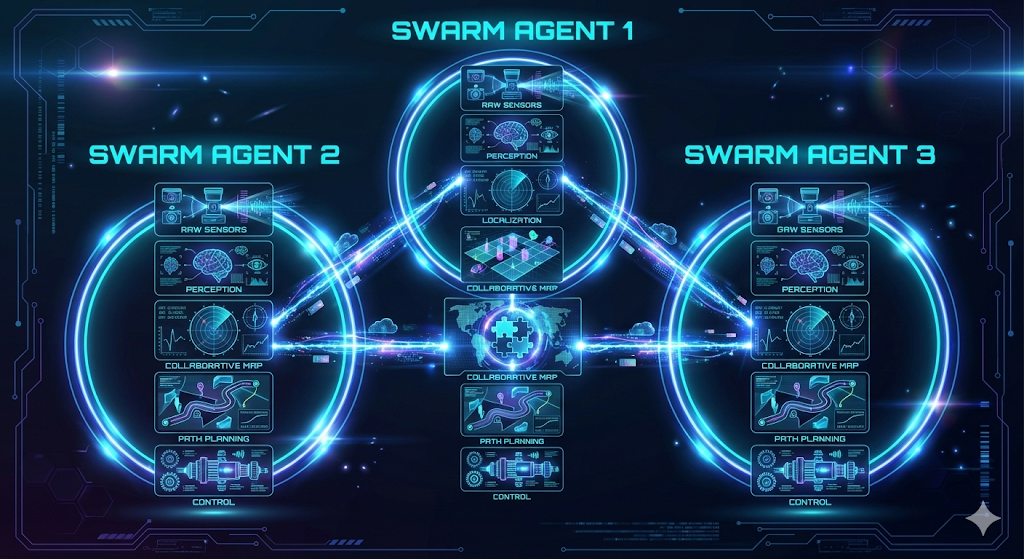
\includegraphics[width=0.85\linewidth]{figures/Chapter 5/High_level_swarm.png}
    \caption{High-Level Swarm Architecture Overview}
    \label{fig:high_level_swarm}
\end{figure}

\subsubsection{Perception Requirements}
The perception module must process dense sensor data in real-time for reliable obstacle avoidance and object detection:
\begin{itemize}
    \item High-resolution LiDAR scans for local costmap construction
    \item Depth camera feeds for dynamic entity detection
    \item Sensor fusion algorithms (Extended Kalman Filter) without latency at 0.2 m/s operating velocity
    \item Neural network inference for on-the-fly object classification
\end{itemize}

\subsubsection{Communication Requirements}
The architecture must support decentralized swarm coordination:
\begin{itemize}
    \item Inter-robot data exchange (telemetry, map fragments, task allocation)
    \item Full-featured OS for network stack and DDS middleware (ROS 2)
    \item Complex message serialization without blocking navigation threads
\end{itemize}

\subsubsection{Navigation and Control Requirements}
\begin{itemize}
    \item Global path planning (A*/Dijkstra) through known map data
    \item Local trajectory adjustment for collision avoidance
    \item Omnidirectional velocity computation ($v_x$, $v_y$, $\omega$) at high frequency
    \item Minimal jitter to prevent drift and localization errors
\end{itemize}

\begin{figure}[H]
    \centering
    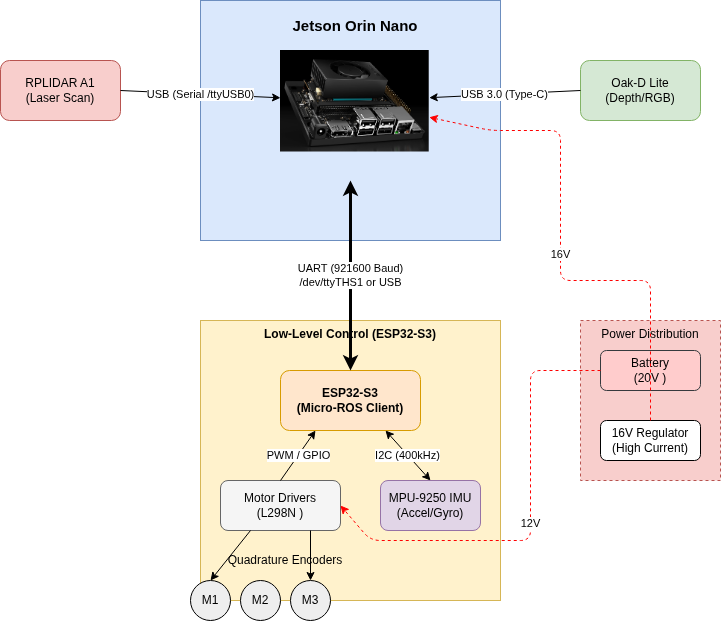
\includegraphics[width=0.8\linewidth]{figures/Chapter 5/Hardware_architecture.png}
    \caption{Hardware Architecture Block Diagram}
    \label{fig:hardware_architecture}
\end{figure}

\subsection{Computing Platform Analysis}
\label{subsec:computing_analysis}

Two leading embedded computing platforms were evaluated: Raspberry Pi 5 and NVIDIA Jetson Orin Nano.

\subsubsection{Raspberry Pi 5}

\begin{figure}[H]
    \centering
    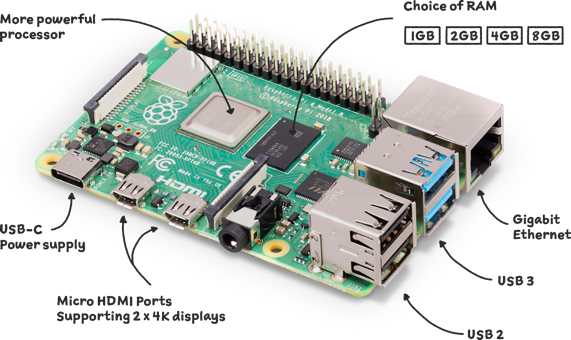
\includegraphics[width=0.5\linewidth]{figures/Chapter 5/Raspbery_pi_5.png}
    \caption{Raspberry Pi 5}
    \label{fig:raspberry_pi}
\end{figure}

The Raspberry Pi 5 represents the standard for general-purpose embedded computing:

\paragraph{Strengths}
\begin{itemize}
    \item Quad-core ARM Cortex-A76 processor
    \item Versatile I/O: dual HDMI, Gigabit Ethernet, USB 3.0, 40-pin GPIO
    \item Massive community support and mature Debian-based OS
    \item Simplified ROS 2 installation
\end{itemize}

\paragraph{Limitations}
\begin{itemize}
    \item No hardware acceleration for AI/ML workloads
    \item CPU-bound processing for point clouds and neural networks
    \item VideoCore GPU designed for multimedia, not parallel computing
    \item Thermal throttling under sustained heavy loads causes latency spikes
\end{itemize}

\subsubsection{NVIDIA Jetson Orin Nano}

\begin{figure}[H]
    \centering
    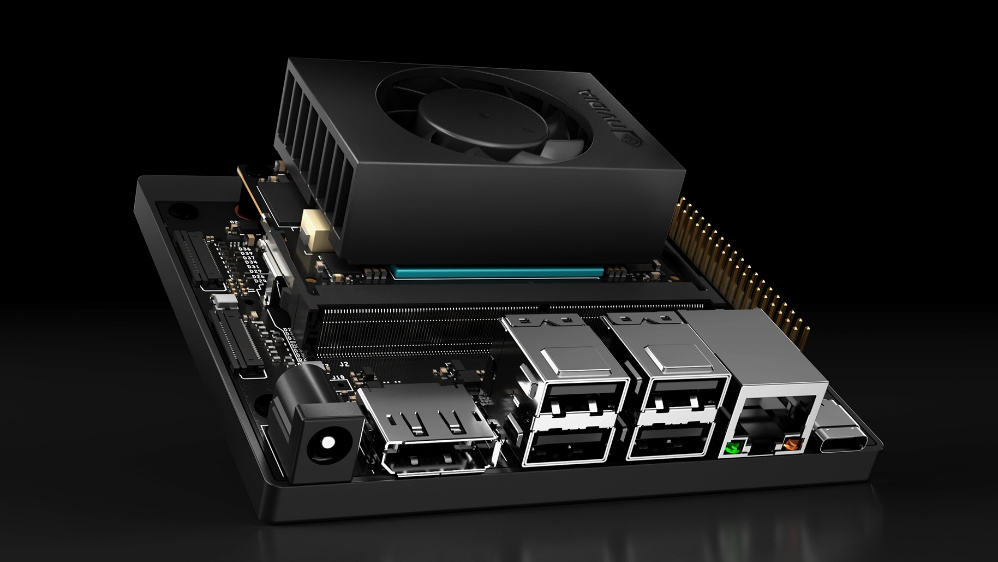
\includegraphics[width=0.5\linewidth]{figures/Chapter 5/Jetson_orin_nano.jpg}
    \caption{NVIDIA Jetson Orin Nano Development Kit}
    \label{fig:jetson_orin}
\end{figure}

The Jetson Orin Nano is engineered specifically for edge AI and autonomous robotics:

\paragraph{Strengths}
\begin{itemize}
    \item NVIDIA Ampere GPU: 1024 CUDA cores, 32 Tensor Cores
    \item Up to 40 TOPS AI performance
    \item 6-core ARM Cortex-A78AE processor
    \item M.2 Key M for NVMe SSD support
    \item JetPack SDK with CUDA-X, TensorRT, and ISAAC ROS libraries
    \item Development kit includes heatsink and fan assembly
\end{itemize}

\paragraph{Limitations}
\begin{itemize}
    \item Higher cost and complexity
    \item Requires carrier board and robust power supply
    \item Increased power consumption during GPU operations
    \item Larger thermal solution adds to physical footprint
\end{itemize}

\subsection{Platform Selection}
\label{subsec:platform_selection}

\begin{figure}[H]
    \centering
    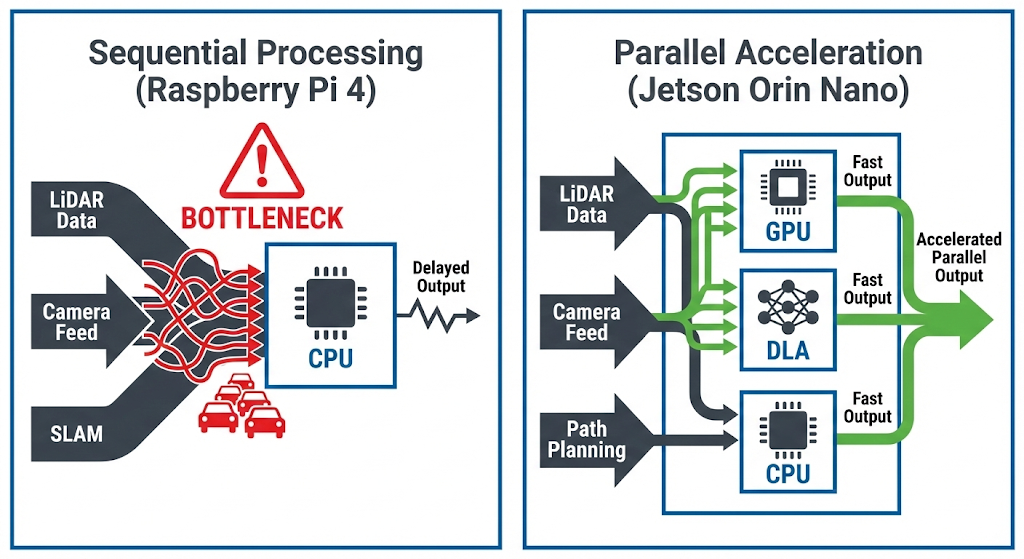
\includegraphics[width=0.75\linewidth]{figures/Chapter 5/pi5_vs_jetson_comparison.png}
    \caption{Raspberry Pi 5 vs. Jetson Orin Nano Comparison}
    \label{fig:pi_vs_jetson}
\end{figure}

The \textbf{NVIDIA Jetson Orin Nano} was selected as the high-level controller for the following reasons \cite{nvidia2023jetson}:

\begin{enumerate}
    \item \textbf{SLAM and Object Detection:} The Raspberry Pi's sequential CPU processing is insufficient for simultaneous localization, mapping, and real-time inference.
    
    \item \textbf{Perception Pipeline:} GPU-accelerated capabilities ensure latency-free processing of dense LiDAR data and neural network models.
    
    \item \textbf{Development Environment:} Ample memory bandwidth supports the full ROS 2 desktop environment and debugging tools directly on the robot.
    
    \item \textbf{Future-Proofing:} The hardware architecture ensures computing capacity does not become the limiting factor as swarm intelligence complexity increases.
\end{enumerate}

\subsection{Depth Camera Selection}
\label{subsec:depth_camera}

Visual perception enables environmental understanding beyond proprioceptive sensors, supporting obstacle detection, visual odometry, robot tracking for swarm coordination, and object recognition.

\subsubsection{Camera Technology Comparison}

\begin{figure}[H]
    \centering
    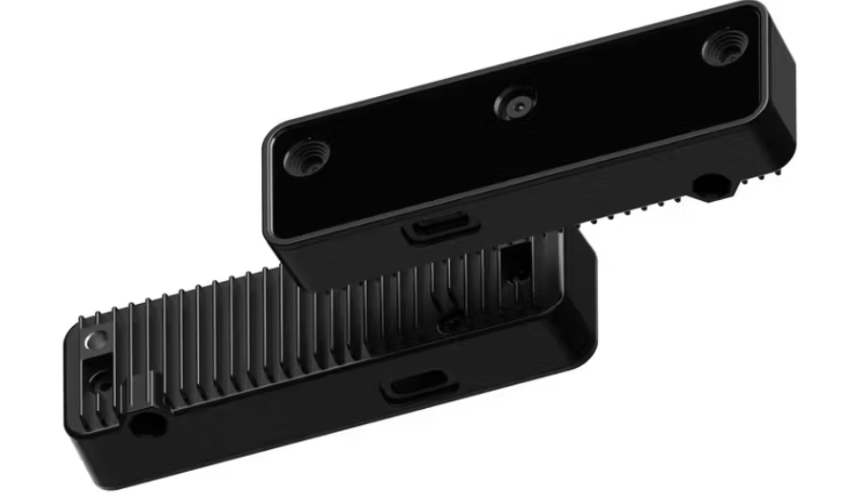
\includegraphics[width=0.6\linewidth]{figures/Chapter 5/cam_1.png}
    \caption{Luxonis OAK-D Lite Depth Camera}
    \label{fig:oakd_lite}
\end{figure}

Four camera technologies were evaluated: monocular RGB, stereo depth, Time-of-Flight (ToF), and structured light.

\begin{table}[H]
\centering
\caption{Camera Configuration Selection Matrix}
\label{tab:camera_config}
\begin{tabular}{|l|c|c|c|c|}
\hline
\textbf{Criteria} & \textbf{Weight} & \textbf{RGB} & \textbf{Stereo Depth} & \textbf{ToF} \\
\hline
Depth Accuracy & 5 & 5 & 20 & 25 \\
\hline
Depth Range & 4 & 4 & 20 & 12 \\
\hline
Computational Efficiency & 4 & 20 & 12 & 20 \\
\hline
Cost & 4 & 20 & 16 & 8 \\
\hline
Environmental Robustness & 3 & 12 & 12 & 9 \\
\hline
Size \& Weight & 2 & 10 & 8 & 8 \\
\hline
\textbf{Final Score} & & \textbf{71} & \textbf{88} & \textbf{82} \\
\hline
\end{tabular}
\end{table}

\subsubsection{Depth Camera Model Comparison}

Three depth camera models were evaluated for the stereo depth configuration:

\begin{figure}[H]
    \centering
    \begin{subfigure}[b]{0.3\textwidth}
        \centering
        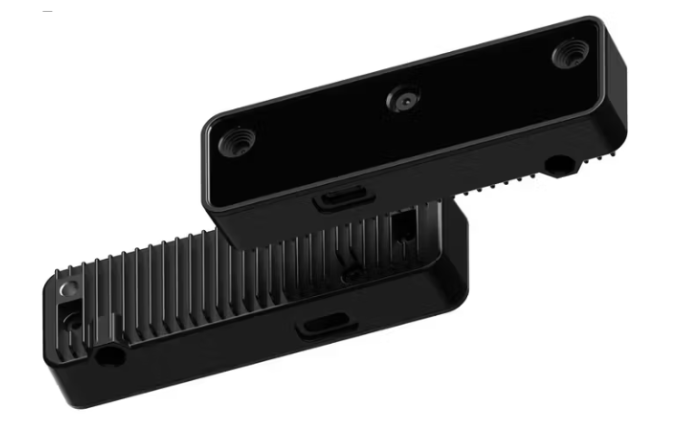
\includegraphics[width=\linewidth]{figures/Chapter 5/cam_4.png}
        \caption{OAK-D Lite}
        \label{fig:oakd_compare}
    \end{subfigure}
    \hfill
    \begin{subfigure}[b]{0.3\textwidth}
        \centering
        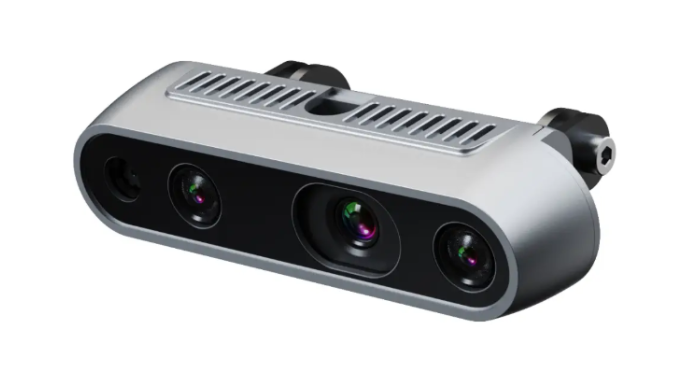
\includegraphics[width=\linewidth]{figures/Chapter 5/cam_5.png}
        \caption{Intel RealSense D435i}
        \label{fig:realsense_compare}
    \end{subfigure}
    \hfill
    \begin{subfigure}[b]{0.3\textwidth}
        \centering
        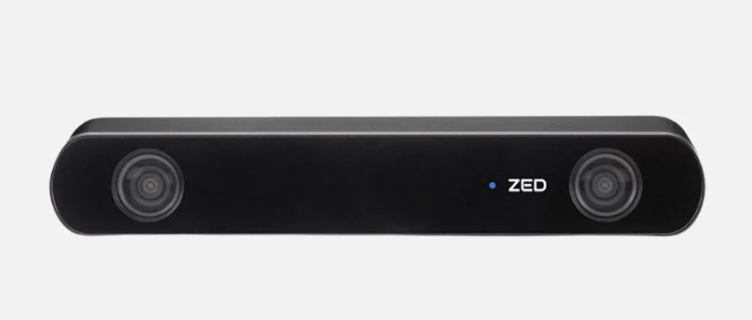
\includegraphics[width=\linewidth]{figures/Chapter 5/cam_6.png}
        \caption{ZED 2i}
        \label{fig:zed_compare}
    \end{subfigure}
    \caption{Depth Camera Candidates}
    \label{fig:depth_camera_candidates}
\end{figure}

\begin{table}[H]
\centering
\caption{Depth Camera Selection Matrix}
\label{tab:depth_camera_selection}
\begin{tabular}{|l|c|c|c|c|}
\hline
\textbf{Criteria} & \textbf{Weight} & \textbf{OAK-D Lite} & \textbf{RealSense D435i} & \textbf{ZED 2i} \\
\hline
Depth Performance & 5 & 20 & 20 & 25 \\
\hline
Onboard AI Processing & 4 & 20 & 4 & 12 \\
\hline
Cost Effectiveness & 4 & 20 & 12 & 8 \\
\hline
Size \& Weight & 3 & 15 & 12 & 9 \\
\hline
Software Ecosystem & 4 & 16 & 20 & 16 \\
\hline
Power Consumption & 3 & 15 & 12 & 9 \\
\hline
Multi-Robot Compatibility & 3 & 15 & 12 & 9 \\
\hline
\textbf{Final Score} & & \textbf{121} & \textbf{92} & \textbf{88} \\
\hline
\end{tabular}
\end{table}

\subsubsection{Final Selection: Luxonis OAK-D Lite}

The \textbf{OAK-D Lite} was selected based on \cite{luxonis2023oakd}:
\begin{enumerate}
    \item \textbf{Onboard AI Processing:} The Intel Myriad X VPU performs depth calculation and neural network inference locally, reducing latency and offloading computation from the Jetson.
    \item \textbf{Cost Advantage:} At approximately half the price of competitors, enables scaling to larger swarms within budget constraints.
    \item \textbf{Adequate Depth Performance:} 2--5 cm accuracy at 1 meter meets navigation requirements with appropriate safety margins.
    \item \textbf{Compact Form Factor:} 96.3 mm × 28.5 mm × 17.2 mm at 62 grams simplifies mechanical integration.
    \item \textbf{ROS 2 Integration:} The \texttt{depthai-ros} package provides excellent support with active development.
\end{enumerate}

\subsubsection{Hardware Specifications}

\begin{itemize}
    \item \textbf{Stereo Cameras:} Dual 1MP (1280×800) global shutter monochrome, 7.5 cm baseline
    \item \textbf{RGB Camera:} 4K (4056×3040) with autofocus
    \item \textbf{Depth Range:} 0.2--20 m (effective 0.5--10 m for indoor operation)
    \item \textbf{Field of View:} 71.9° × 56.6° (stereo), 68.8° × 55.5° (RGB)
    \item \textbf{Depth FPS:} Up to 60 fps at lower resolutions
    \item \textbf{Power:} 2.5W typical via USB 3.1 Type-C
    \item \textbf{AI Performance:} Myriad X VPU supports TensorFlow, PyTorch, OpenVINO models
\end{itemize}

\begin{figure}[H]
    \centering
    \begin{subfigure}[b]{0.45\textwidth}
        \centering
        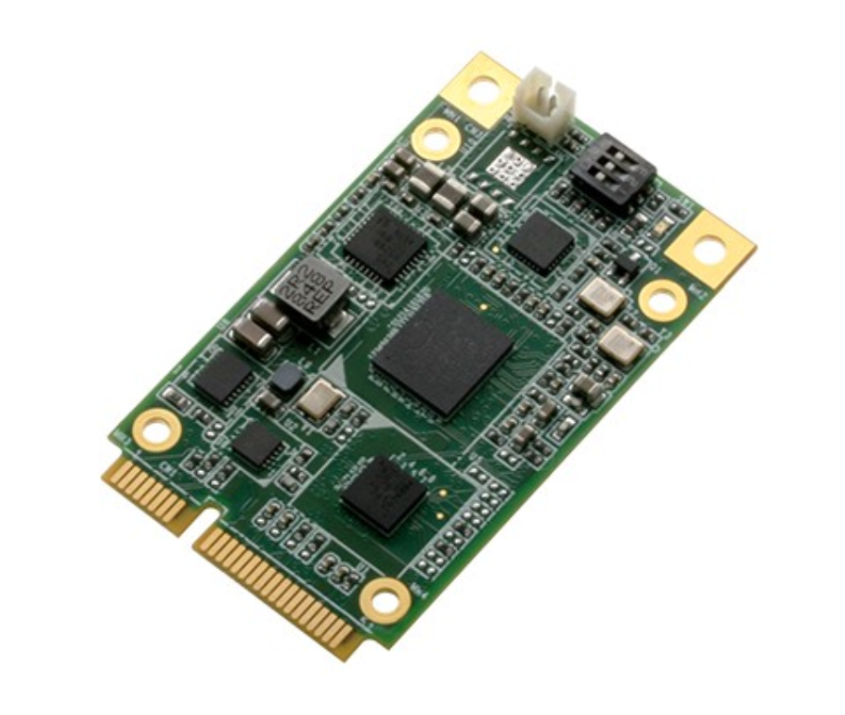
\includegraphics[width=\linewidth]{figures/Chapter 5/cam_2.png}
        \caption{OAK-D Lite System Architecture}
        \label{fig:oakd_architecture}
    \end{subfigure}
    \hfill
    \begin{subfigure}[b]{0.45\textwidth}
        \centering
        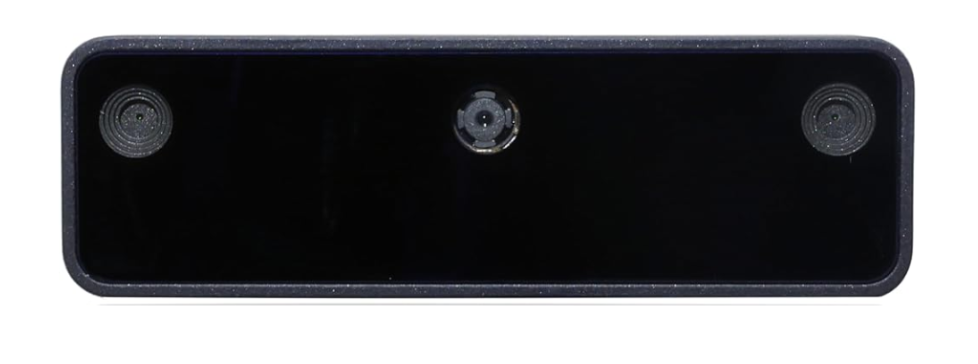
\includegraphics[width=\linewidth]{figures/Chapter 5/cam_3.png}
        \caption{Stereo Camera Configuration}
        \label{fig:stereo_config}
    \end{subfigure}
    \caption{OAK-D Lite Hardware Overview}
    \label{fig:oakd_hardware}
\end{figure}

\subsubsection{Application Scenarios}

\paragraph{Obstacle Detection and Collision Avoidance}
The depth image provides dense 3D point clouds for local occupancy maps, enabling detection of obstacles at varying heights---including overhanging objects and low barriers---that 2D LiDAR cannot capture.

\paragraph{Visual Odometry}
Feature tracking between frames provides independent velocity estimates, validating wheel encoder data during slip conditions when encoders report false movement.

\paragraph{Robot Detection and Swarm Coordination}
Neural network-based detection identifies teammate robots for formation control and collision avoidance, with depth providing direct 3D position relative to the detecting robot.

\paragraph{Semantic Scene Understanding}
Pixel-level classification (floor, wall, furniture, objects) supports task planning, while object recognition enables manipulation tasks for warehouse automation or search and rescue operations.

\begin{figure}[H]
    \centering
    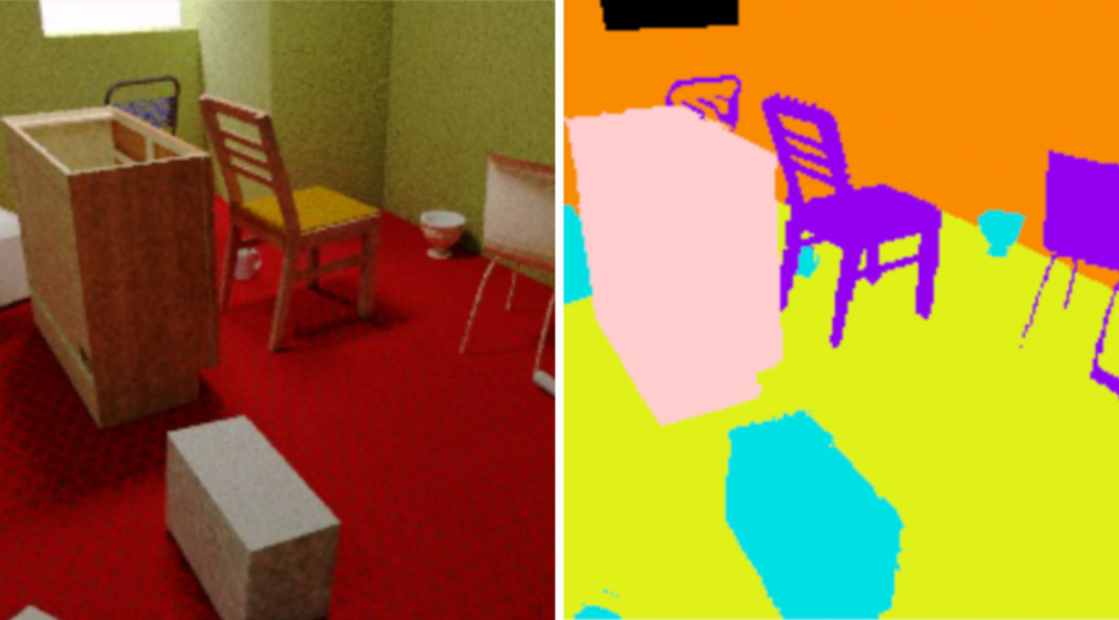
\includegraphics[width=0.7\linewidth]{figures/Chapter 5/cam_7.png}
    \caption{Semantic Segmentation Example}
    \label{fig:semantic_segmentation}
\end{figure}

\subsubsection{Mechanical Integration}

A custom 3D-printed PLA+ mounting bracket positions the camera at an elevated location maximizing forward and lateral field of view while maintaining structural rigidity. The mount resists vibration during robot operation and maintains stereo pair alignment for accurate depth calculation.

\begin{figure}[H]
    \centering
    \begin{subfigure}[b]{0.45\textwidth}
        \centering
        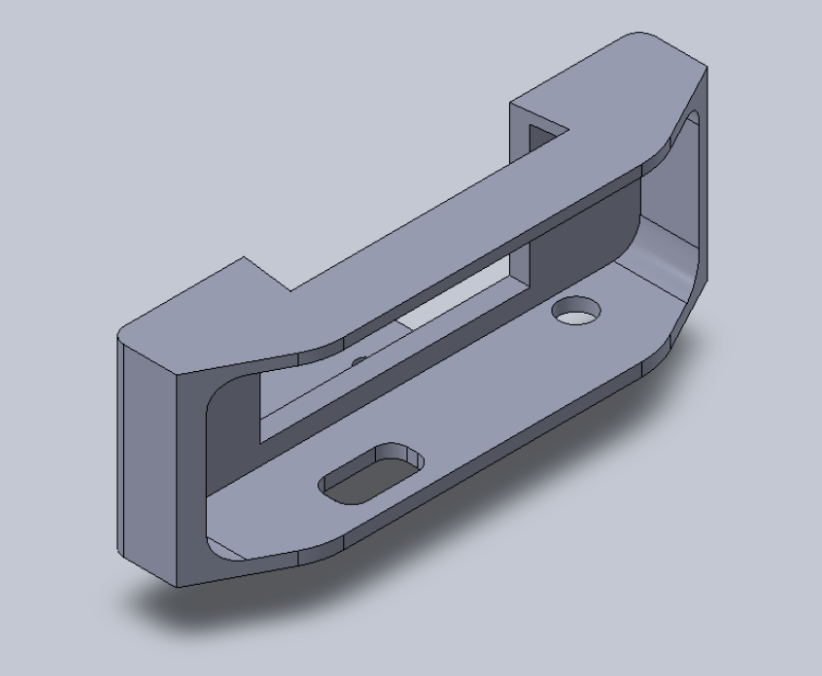
\includegraphics[width=\linewidth]{figures/Chapter 5/cam_8.png}
        \caption{Camera Mount Design}
        \label{fig:cam_mount_design}
    \end{subfigure}
    \hfill
    \begin{subfigure}[b]{0.45\textwidth}
        \centering
        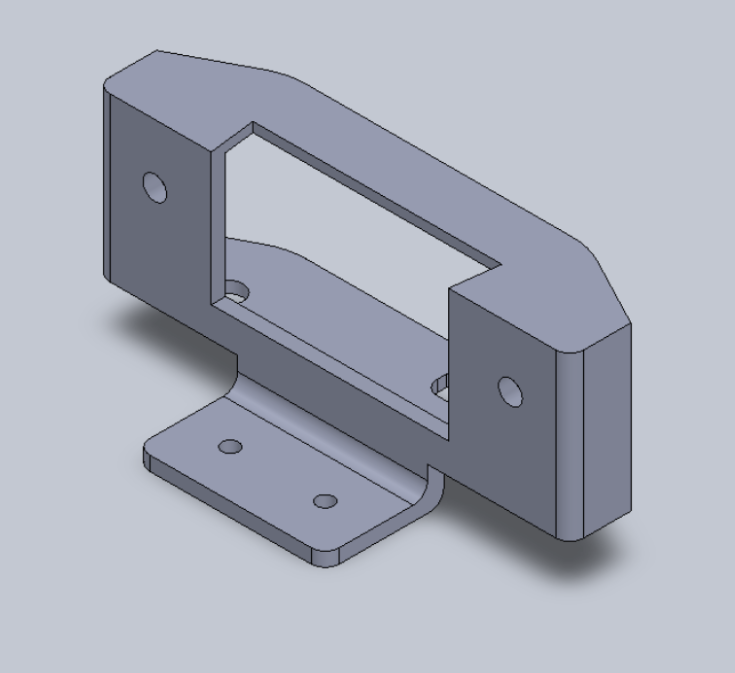
\includegraphics[width=\linewidth]{figures/Chapter 5/cam_9.png}
        \caption{Installed Camera Mount}
        \label{fig:cam_mount_installed}
    \end{subfigure}
    \caption{OAK-D Lite Mechanical Mounting}
    \label{fig:camera_mounting}
\end{figure}

\subsection{Inertial Measurement Unit Selection}
\label{subsec:imu_selection}

The IMU provides high-frequency measurements (100 Hz) of orientation, angular velocity, and linear acceleration---critical for navigation when other sensors are unavailable or compromised. It operates independently of environmental conditions, making it valuable during rapid rotations, dusty conditions, or areas with poor visual features.

\begin{figure}[H]
    \centering
    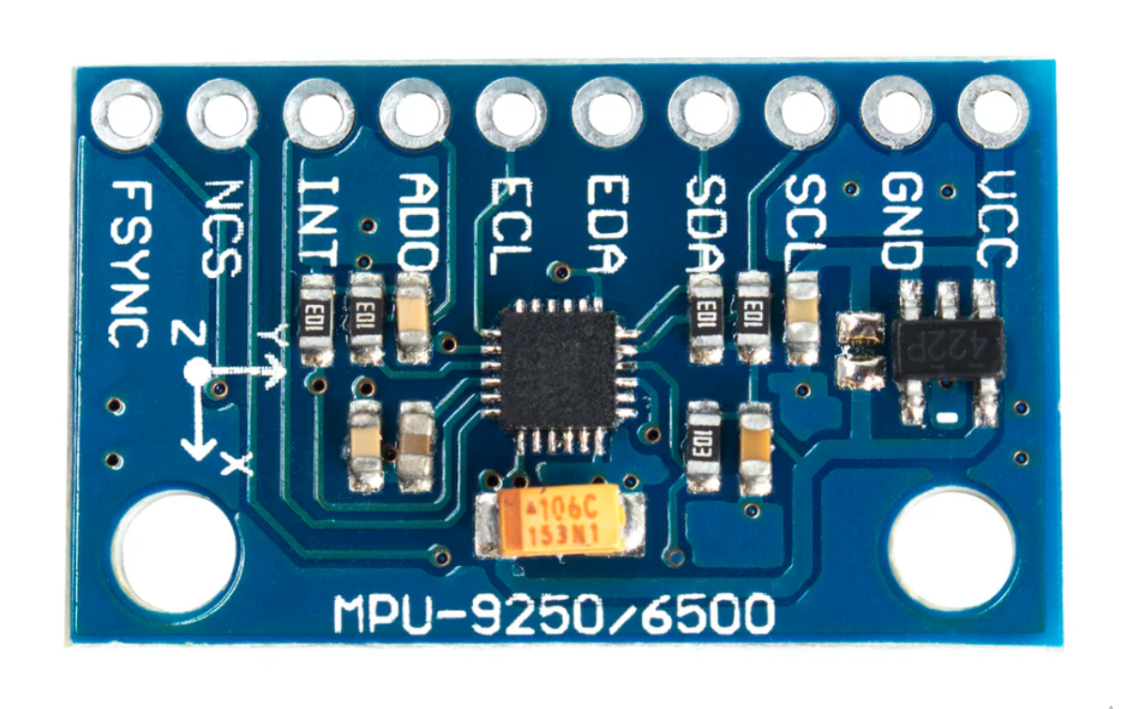
\includegraphics[width=0.5\linewidth]{figures/Chapter 5/IMU_image.png}
    \caption{MPU-9250 9-Axis IMU Module}
    \label{fig:imu_module}
\end{figure}

\subsubsection{IMU Configuration Comparison}

Three IMU configurations were evaluated: 6-axis (gyroscope + accelerometer), 9-axis (with magnetometer), and sensor fusion IMUs (with onboard processing).

\begin{table}[H]
\centering
\caption{IMU Configuration Selection Matrix}
\label{tab:imu_config}
\begin{tabular}{|l|c|c|c|c|}
\hline
\textbf{Criteria} & \textbf{Weight} & \textbf{6-Axis} & \textbf{9-Axis} & \textbf{Fusion IMU} \\
\hline
Accuracy \& Performance & 5 & 20 & 20 & 25 \\
\hline
Cost & 4 & 20 & 16 & 8 \\
\hline
Software Ecosystem & 4 & 16 & 20 & 16 \\
\hline
Size \& Weight & 3 & 15 & 15 & 9 \\
\hline
Power Consumption & 3 & 15 & 12 & 9 \\
\hline
Magnetometer Benefit & 2 & 2 & 10 & 10 \\
\hline
\textbf{Final Score} & & \textbf{88} & \textbf{93} & \textbf{67} \\
\hline
\end{tabular}
\end{table}

\subsubsection{IMU Model Comparison}

Three 9-axis IMU models were evaluated:

\begin{table}[H]
\centering
\caption{IMU Model Selection Matrix}
\label{tab:imu_model}
\begin{tabular}{|l|c|c|c|c|}
\hline
\textbf{Criteria} & \textbf{Weight} & \textbf{MPU-9250} & \textbf{BNO055} & \textbf{ICM-20948} \\
\hline
Sensor Performance & 5 & 20 & 25 & 25 \\
\hline
Cost-Effectiveness & 4 & 20 & 8 & 12 \\
\hline
Size \& Weight & 3 & 12 & 9 & 12 \\
\hline
Software Ecosystem & 4 & 20 & 16 & 12 \\
\hline
Power Consumption & 3 & 12 & 12 & 12 \\
\hline
Availability & 3 & 15 & 6 & 3 \\
\hline
\textbf{Final Score} & & \textbf{99} & \textbf{76} & \textbf{76} \\
\hline
\end{tabular}
\end{table}

\subsubsection{Final Selection: MPU-9250}

The \textbf{MPU-9250} was selected based on:
\begin{enumerate}
    \item \textbf{Software Ecosystem:} Extensive Arduino libraries, ROS drivers, and calibration tools with strong community support.
    \item \textbf{Cost Advantage:} At \$15--20 per unit (vs. \$35--45 for BNO055), enables 10-robot swarms for the cost of 4--5 premium-IMU robots.
    \item \textbf{Adequate Performance:} Gyroscope noise density 0.01°/s/$\sqrt{\text{Hz}}$, accelerometer noise density 300 $\mu$g/$\sqrt{\text{Hz}}$---sufficient for mobile robot navigation with EKF fusion.
    \item \textbf{I2C Compatibility:} 3.3V operation compatible with both ESP32-S3 (prototyping) and Jetson Orin Nano (production).
\end{enumerate}

\subsubsection{Hardware Specifications}

\begin{itemize}
    \item \textbf{Gyroscope:} 3-axis, $\pm$2000°/s range, 16-bit ADC
    \item \textbf{Accelerometer:} 3-axis, $\pm$16g range, 16-bit ADC
    \item \textbf{Magnetometer:} 3-axis, $\pm$4800 $\mu$T range
    \item \textbf{Interface:} I2C at 400 kHz (Fast Mode)
    \item \textbf{Update Rate:} 100 Hz configured
    \item \textbf{Power:} 3.3V, low consumption
\end{itemize}

\subsubsection{Hardware Implementation}

\begin{figure}[H]
    \centering
    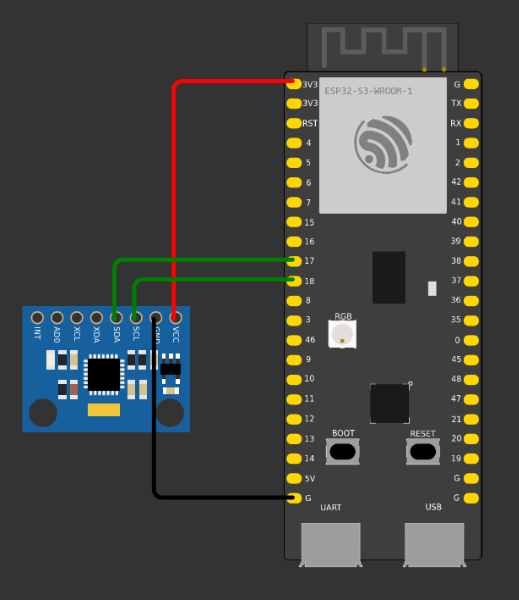
\includegraphics[width=0.6\linewidth]{figures/Chapter 5/IMU_circuit_schematic.png}
    \caption{IMU I2C Connection Schematic}
    \label{fig:imu_schematic}
\end{figure}

A custom interface PCB was developed for mechanical stability and maintenance:
\begin{itemize}
    \item \textbf{Header-Based Interface:} 5-pin configuration (VCC, GND, SCL, SDA, EDA) for quick sensor swapping
    \item \textbf{Terminal Blocks:} Screw-type connectors prevent vibration-induced disconnections
    \item \textbf{Rigid Mounting:} M3 bolts secure PCB to chassis, maintaining alignment with \texttt{base\_link} frame
\end{itemize}

\begin{figure}[H]
    \centering
    \begin{subfigure}[b]{0.3\textwidth}
        \centering
        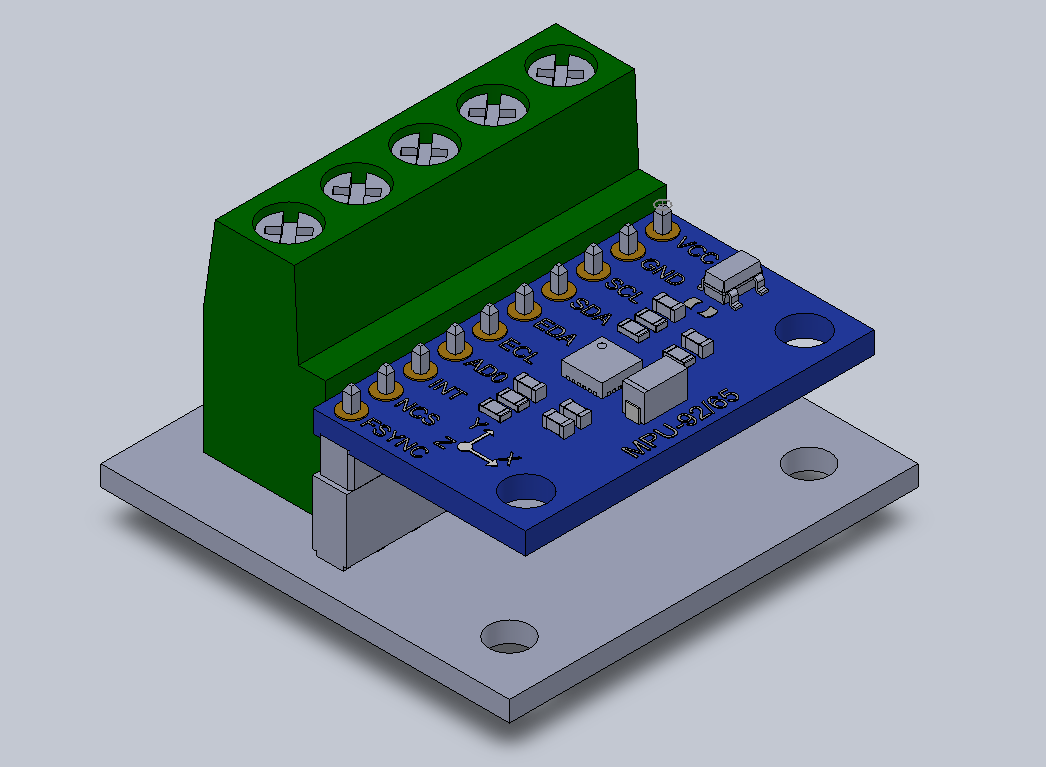
\includegraphics[width=\linewidth]{figures/Chapter 5/IMU_pcb_1.png}
        \caption{PCB Design}
        \label{fig:imu_pcb1}
    \end{subfigure}
    \hfill
    \begin{subfigure}[b]{0.3\textwidth}
        \centering
        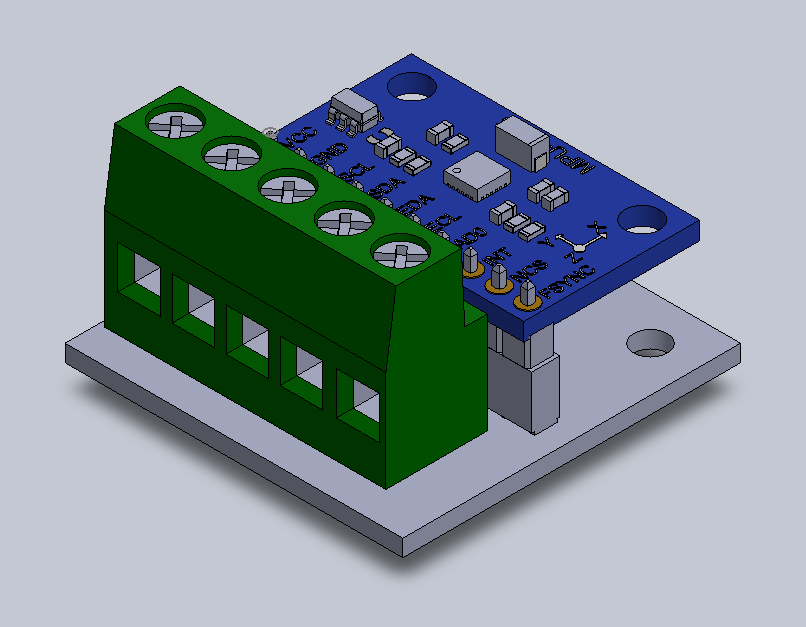
\includegraphics[width=\linewidth]{figures/Chapter 5/IMU_pcb_2.png}
        \caption{Assembled PCB}
        \label{fig:imu_pcb2}
    \end{subfigure}
    \hfill
    \begin{subfigure}[b]{0.3\textwidth}
        \centering
        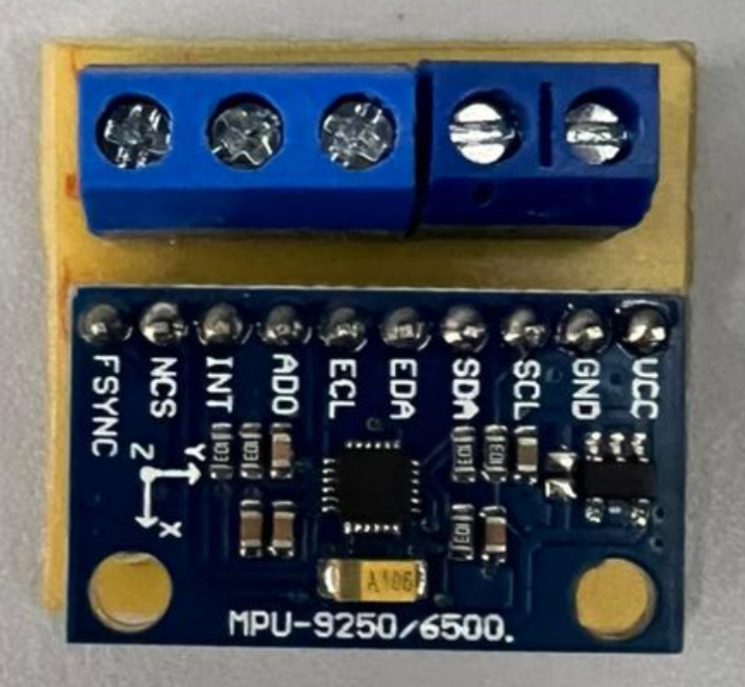
\includegraphics[width=\linewidth]{figures/Chapter 5/IMU_pcb_3.png}
        \caption{Mounted Assembly}
        \label{fig:imu_pcb3}
    \end{subfigure}
    \caption{IMU Custom Interface PCB}
    \label{fig:imu_pcb}
\end{figure}

\subsubsection{Calibration Procedures}

\paragraph{Accelerometer and Gyroscope Calibration}
At startup, 500 samples are collected with the sensor stationary on a horizontal surface. Outliers ($>$2$\sigma$ from mean) are rejected before averaging to determine bias values.

\paragraph{Magnetometer Calibration}
Requires rotation through full range of orientations to characterize hard-iron offsets (constant fields) and soft-iron distortions. A standardized figure-eight procedure for 20 seconds around each axis ensures consistent calibration.

\subsection{LiDAR Selection}
\label{subsec:lidar_selection}

The primary exteroceptive sensor provides geometric perception of the environment through laser scanning. LiDAR measures distance using Time-of-Flight (ToF) principles: a laser pulse is emitted at time $t_0$, reflects off obstacles, and returns at time $t_1$. The distance is calculated as:
\begin{equation}
d = \frac{c \cdot \Delta t}{2}
\label{eq:lidar_distance}
\end{equation}
where $c$ is the speed of light and $\Delta t = t_1 - t_0$.

The output in polar coordinates $(r, \theta)$ is converted to Cartesian coordinates:
\begin{equation}
x_{robot} = r \cdot \cos(\theta), \quad y_{robot} = r \cdot \sin(\theta)
\label{eq:lidar_cartesian}
\end{equation}

\subsubsection{2D vs. 3D LiDAR Comparison}

\begin{table}[H]
\centering
\caption{LiDAR Type Selection Matrix}
\label{tab:lidar_type}
\begin{tabular}{|l|c|c|c|c|c|}
\hline
\textbf{Criteria} & \textbf{Weight} & \multicolumn{2}{c|}{\textbf{2D LiDAR}} & \multicolumn{2}{c|}{\textbf{3D LiDAR}} \\
\cline{3-6}
 & & Rating & Score & Rating & Score \\
\hline
Swarm Scalability (Cost) & 5 & 5 & 25 & 0 & 0 \\
\hline
Field of View (FOV) & 5 & 5 & 25 & 5 & 25 \\
\hline
Computational Efficiency & 4 & 5 & 20 & 1 & 4 \\
\hline
Range \& Accuracy & 3 & 3 & 9 & 5 & 15 \\
\hline
ROS 2 Integration & 3 & 5 & 15 & 5 & 15 \\
\hline
\textbf{Final Score} & & & \textbf{94} & & \textbf{59} \\
\hline
\end{tabular}
\end{table}

\subsubsection{Final Selection: RPLIDAR A1}

\begin{figure}[H]
    \centering
    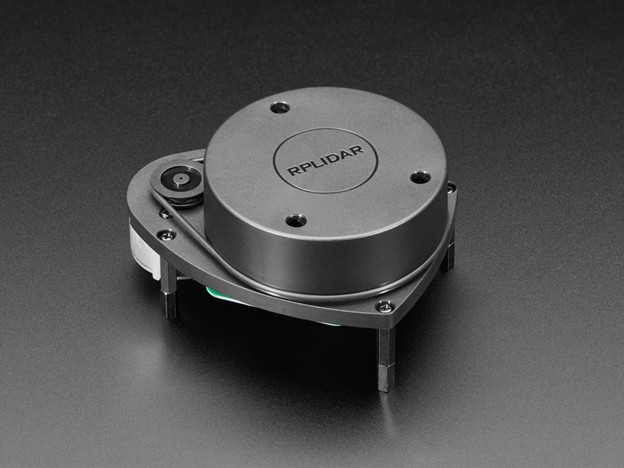
\includegraphics[width=0.4\linewidth]{figures/Chapter 5/rplidar.jpg}
    \caption{RPLIDAR A1 360-Degree 2D Laser Scanner}
    \label{fig:rplidar}
\end{figure}

The \textbf{RPLIDAR A1} was selected based on \cite{slamtec2023rplidar}:
\begin{itemize}
    \item \textbf{360° FOV:} Complete environmental awareness in a single scan
    \item \textbf{Cost-Effective:} Enables swarm scalability at \$99 per unit
    \item \textbf{Sufficient Range:} 12m range adequate for indoor navigation
    \item \textbf{Low Computational Load:} 2D point clouds enable real-time SLAM on embedded platforms
    \item \textbf{Mature ROS 2 Support:} Official SLAMTEC driver package
\end{itemize}

\paragraph{Hardware Specifications}
\begin{itemize}
    \item \textbf{Range:} 0.15--12 m
    \item \textbf{Angular Resolution:} $<$1° (5.5 Hz scan rate)
    \item \textbf{Scan Rate:} 5.5--10 Hz configurable
    \item \textbf{Interface:} USB (Serial/UART)
    \item \textbf{Power:} 5V, 500mA typical
\end{itemize}

\subsubsection{ROS 2 Integration}

\paragraph{Hardware Driver}
The official SLAMTEC ROS 2 driver provides hardware abstraction:
\begin{itemize}
    \item Communicates via USB serial
    \item Controls motor speed (PWM)
    \item Parses raw byte stream into \texttt{sensor\_msgs/LaserScan}
\end{itemize}

\paragraph{Simulation Driver}
In Gazebo, a ray sensor plugin simulates the LiDAR physics, outputting identical \texttt{LaserScan} messages for algorithm development.

\begin{figure}[H]
    \centering
    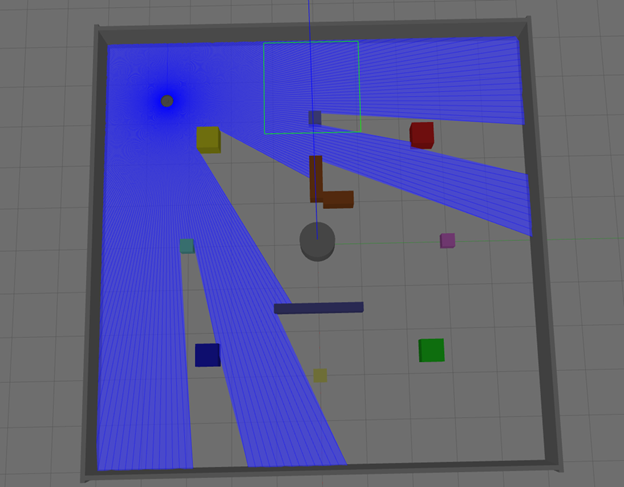
\includegraphics[width=0.7\linewidth]{figures/Chapter 5/lidar_rays_gazebo.png}
    \caption{LiDAR Simulation in Gazebo}
    \label{fig:lidar_gazebo}
\end{figure}

\paragraph{Data Output}
The standardized \texttt{sensor\_msgs/LaserScan} message contains:
\begin{itemize}
    \item \textbf{Header:} Timestamp and \texttt{frame\_id} for TF synchronization
    \item \textbf{Angle Increment:} Angular resolution between beams
    \item \textbf{Ranges Array:} Distance measurements to obstacles
\end{itemize}

\begin{figure}[H]
    \centering
    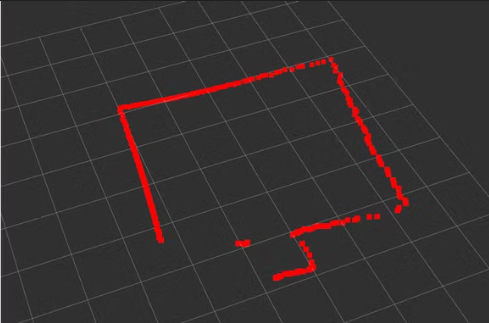
\includegraphics[width=0.7\linewidth]{figures/Chapter 5/lidar_laser_rviz.png}
    \caption{LiDAR Data Visualization in RViz2}
    \label{fig:lidar_rviz}
\end{figure}
\newpage
\section{System Architecture}
\label{sec:system_architecture}

\subsection{Software Stack Overview}
The AUSRA software stack utilizes a containerized approach to ensure portability and reproducibility. The architecture is built upon the Robot Operating System (ROS) framework \cite{quigley2009ros}, specifically ROS 2 Humble, which provides standardized interfaces for sensor integration, inter-process communication, and navigation.

\begin{figure}[H]
    \centering
    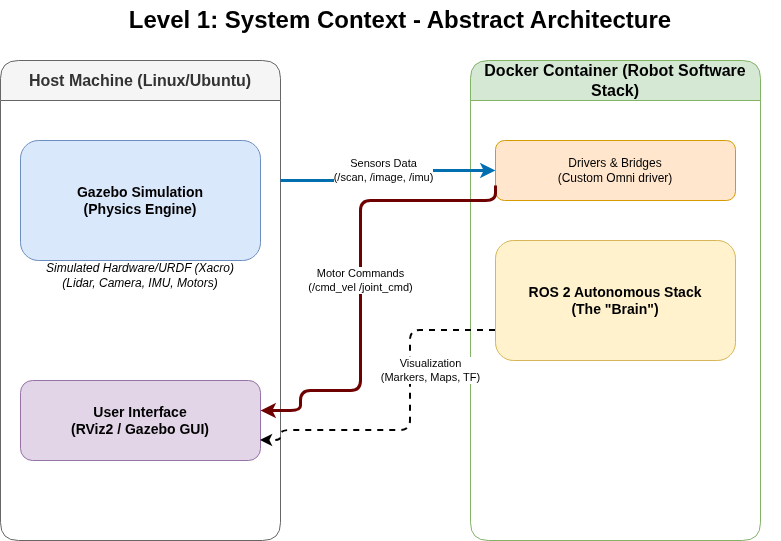
\includegraphics[width=0.9\linewidth]{figures/Chapter 5/Abstract_Architecture.png}
    \caption{Level 1: System Context - Abstract Architecture}
    \label{fig:abstract_arch}
\end{figure}

As illustrated in Figure \ref{fig:abstract_arch}, the architecture separates the simulation host from the robot software:
\begin{itemize}
    \item \textbf{Host Machine:} Runs the Gazebo Physics Engine and RViz2
    \item \textbf{Docker Container:} Encapsulates the complete ``Robot Brain'' (Drivers, SLAM, Nav2, Exploration)
\end{itemize}

\subsection{Key Software Components}
\begin{itemize}
    \item \textbf{Perception:} LiDAR and Depth Camera processing
    \item \textbf{Localization:} AMCL and SLAM Toolbox
    \item \textbf{Planning:} Global (A*) and local (DWB) path planners
    \item \textbf{Exploration:} Frontier-based autonomous mapping
    \item \textbf{Control:} Omnidirectional kinematics
\end{itemize}

\subsection{Low-Level Interface (micro-ROS)}

The system handles real-time hardware control using micro-ROS running on an ESP32-S3 microcontroller. This bridge connects the high-level ROS 2 stack (on the Jetson Orin Nano) with low-level actuators and sensors.

\begin{itemize}
    \item \textbf{Transport:} Communication via UART (Serial) at 921600 baud to minimize latency
    \item \textbf{Architecture:}
    \begin{itemize}
        \item \textbf{Client (ESP32-S3):} Runs the micro-ROS Client, implementing real-time PID loops for motor velocity control and reading raw IMU/Encoder data
        \item \textbf{Agent (Jetson Host):} Runs the \texttt{micro\_ros\_agent}, acting as a DDS proxy, making the embedded device's topics visible to the ROS 2 network
    \end{itemize}
    \item \textbf{Entities:} The ESP32 exposes:
    \begin{itemize}
        \item Subscribers: \texttt{/cmd\_vel} (Twist) for target velocities
        \item Publishers: \texttt{/odom} (Odometry) and \texttt{/imu/raw} (Sensor data)
    \end{itemize}
\end{itemize}

\subsection{Deployment on Jetson Orin Nano (Docker)}

The entire software stack is containerized for reliable deployment on the NVIDIA Jetson Orin Nano:

\begin{itemize}
    \item \textbf{Containerization:} A custom Docker image encapsulates ROS 2 Humble \cite{ros2design2020}, Nav2 \cite{nav2docs, macenski2020marathon2}, SLAM Toolbox, and all dependencies, preventing ``dependency hell'' and ensuring consistent library versions
    \item \textbf{Network Configuration:} Containers use \texttt{network\_mode: host}, allowing DDS middleware to access host network interfaces for multicast discovery---critical for swarm communication
    \item \textbf{Hardware Acceleration:} Docker configured with NVIDIA Container Runtime (\texttt{--runtime nvidia}), granting ROS nodes GPU access for accelerated perception
\end{itemize}

\subsection{Core ROS 2 Node Overview}

The autonomous stack comprises several interconnected ROS 2 nodes, each responsible for a specific function in the perception-planning-control pipeline:

\begin{table}[H]
\centering
\caption{Core ROS 2 Nodes and Their Functions}
\label{tab:ros_nodes}
\begin{tabular}{|l|p{4.5cm}|p{5cm}|}
\hline
\textbf{Node Name} & \textbf{Function} & \textbf{Key Topics} \\
\hline
\texttt{rplidar\_node} & LiDAR data acquisition & Pub: \texttt{/scan} \\
\texttt{imu\_serial\_node} & IMU data acquisition & Pub: \texttt{/imu/data\_raw}, \texttt{/imu/mag} \\
\texttt{ekf\_node} & EKF sensor fusion & Sub: \texttt{/imu/data\_raw}, \texttt{/wheel/odom} \newline Pub: \texttt{/odometry/filtered}, \texttt{/tf} \\
\texttt{slam\_toolbox} & SLAM and mapping & Sub: \texttt{/scan}, \texttt{/tf} \newline Pub: \texttt{/map}, \texttt{/tf} \\
\texttt{bt\_navigator} & Behavior tree navigation & Sub: \texttt{/goal\_pose} \newline Pub: Navigation actions \\
\texttt{planner\_server} & Global path planning (A*) & Pub: \texttt{/plan} \\
\texttt{controller\_server} & Local trajectory control (DWB) & Pub: \texttt{/cmd\_vel} \\
\texttt{omni\_driver} & Inverse kinematics \& odometry & Sub: \texttt{/cmd\_vel} \newline Pub: \texttt{/wheel/odom}, \texttt{/wheel\_cmd} \\
\texttt{micro\_ros\_agent} & ESP32 communication bridge & DDS $\leftrightarrow$ Serial \\
\hline
\end{tabular}
\end{table}

The data flow follows the standard ROS 2 navigation architecture: sensors feed into localization and mapping nodes, which provide the environmental context for the Nav2 planning and control servers, ultimately producing velocity commands executed by the omnidirectional driver.

\section{Simulation Environment}
\label{sec:simulation}

The AUSRA system is validated in a high-fidelity simulation environment using Gazebo Classic. The simulation runs on the host machine and communicates with the autonomous stack (in Docker) via standard ROS 2 interfaces.

\subsection{Testing Scenarios}

Several distinct environments stress-test different aspects of the system:

\begin{itemize}
    \item \textbf{Basic Verification (Rooms 1 \& 2):} Simple, enclosed environments for unit testing navigation, mapping quality, and obstacle avoidance
    \item \textbf{Disaster Response (Office Earthquake):} Complex, unstructured environment representing a collapsed office building with debris, narrow passageways, and clutter \cite{marder2010office}---designed for Frontier Exploration and constrained navigation testing
    \item \textbf{Coordination (Multi-Robot Room):} Large, open environment for swarm testing with multiple agents to verify Collaborative SLAM and decentralized avoidance
\end{itemize}

An example of the semantic construction of these worlds (SDF format) is provided in Appendix \ref{app:sim_code}.

\begin{figure}[H]
    \centering
    \begin{subfigure}[b]{0.48\textwidth}
        \centering
        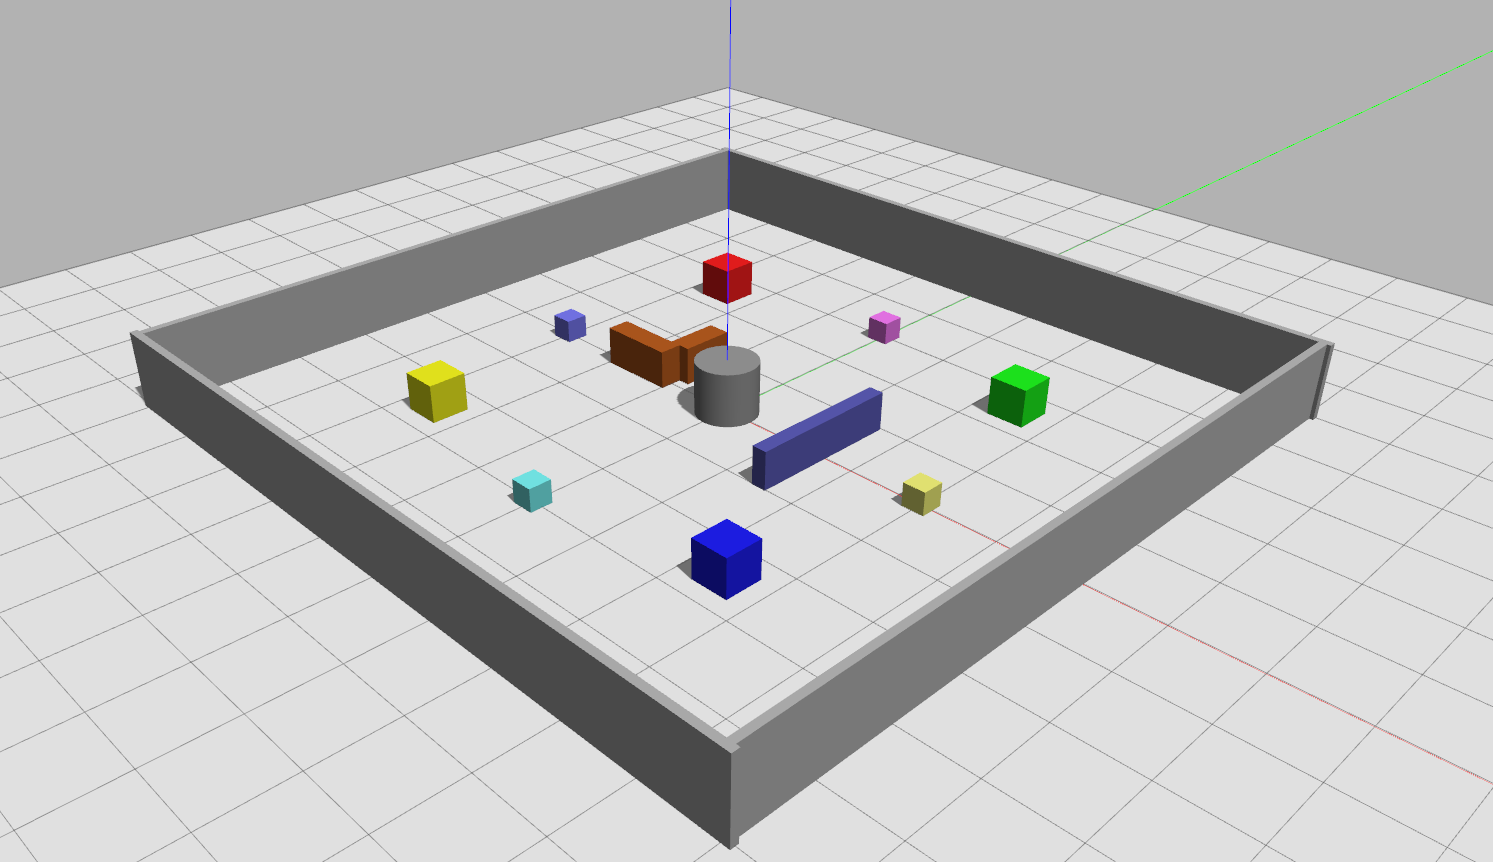
\includegraphics[width=\textwidth]{figures/Chapter 5/Room_1_simualtion.png}
        \caption{Room 1: Basic Verification}
        \label{fig:room1}
    \end{subfigure}
    \hfill
    \begin{subfigure}[b]{0.48\textwidth}
        \centering
        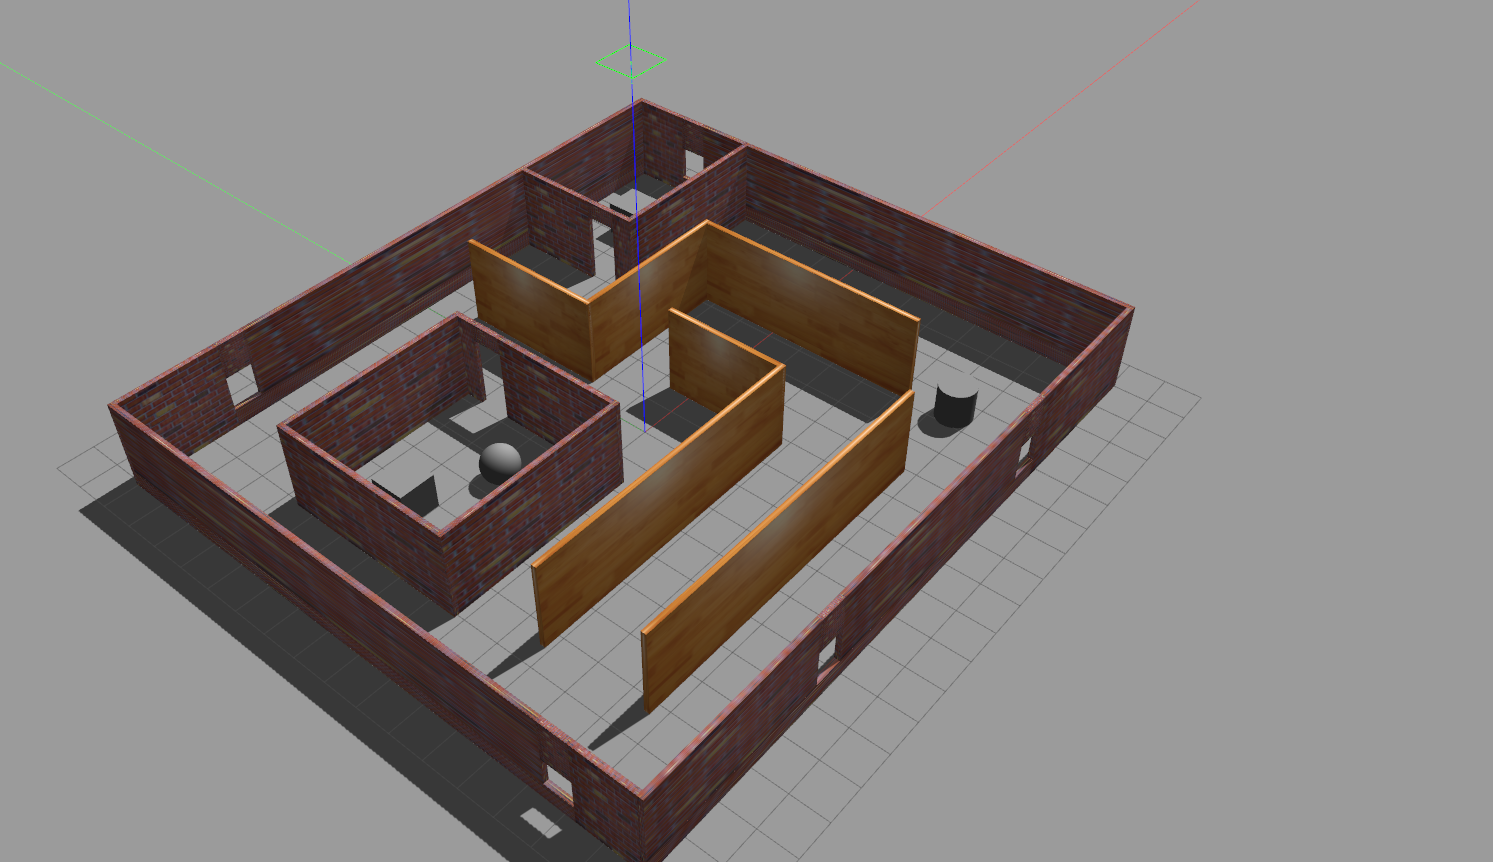
\includegraphics[width=\textwidth]{figures/Chapter 5/Room_2_simulation.png}
        \caption{Room 2: Complex Geometry}
        \label{fig:room2}
    \end{subfigure}
    \caption{Unit Testing Environments}
    \label{fig:test_rooms}
\end{figure}

\begin{figure}[H]
    \centering
    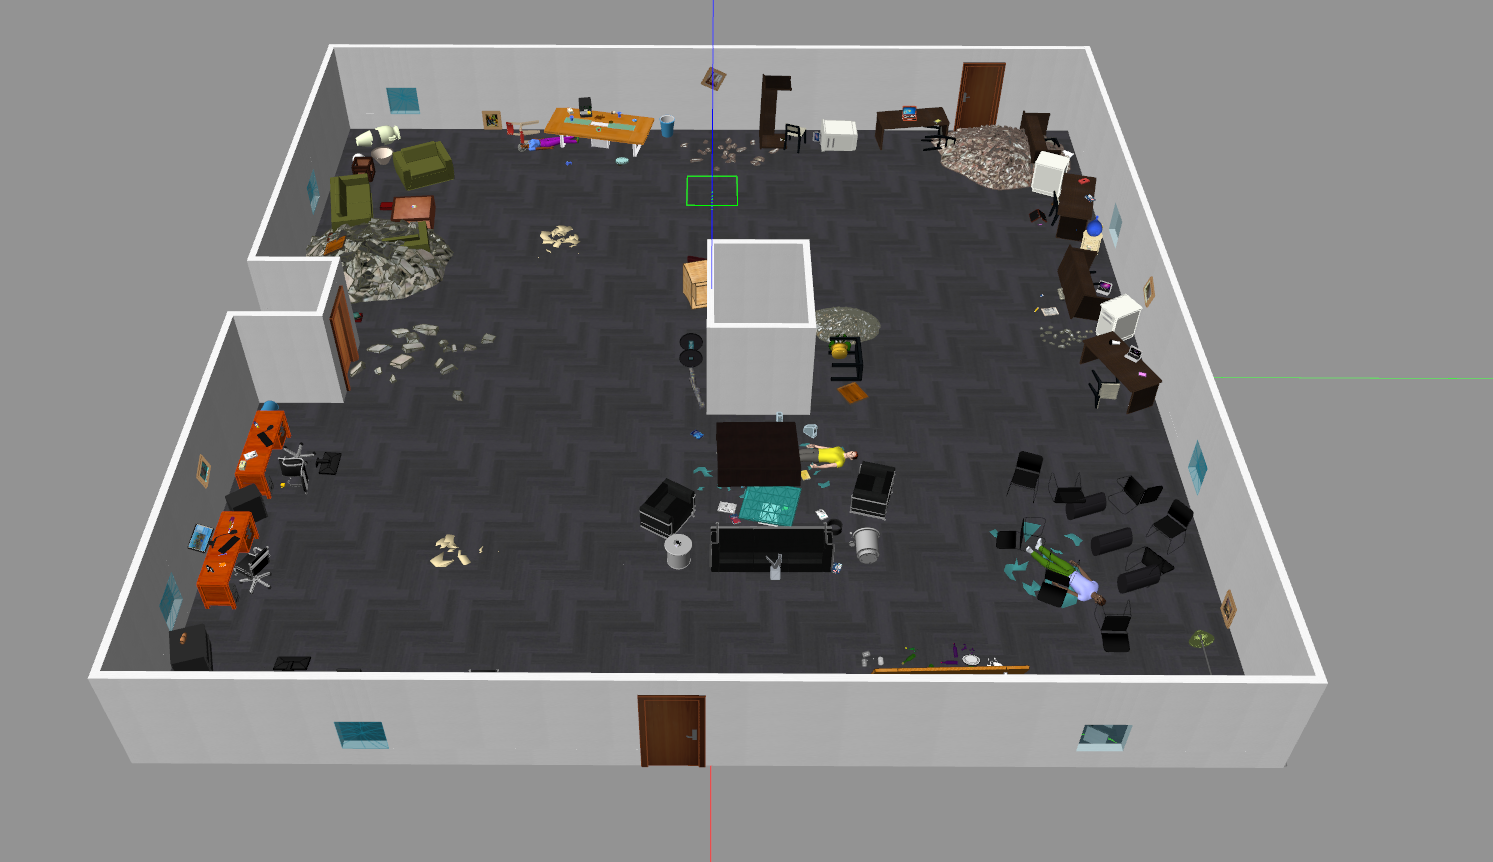
\includegraphics[width=0.9\linewidth]{figures/Chapter 5/office_earthquake_simualtion.png}
    \caption{Office Earthquake World: Disaster Response Scenario}
    \label{fig:earthquake}
\end{figure}

\begin{figure}[H]
    \centering
    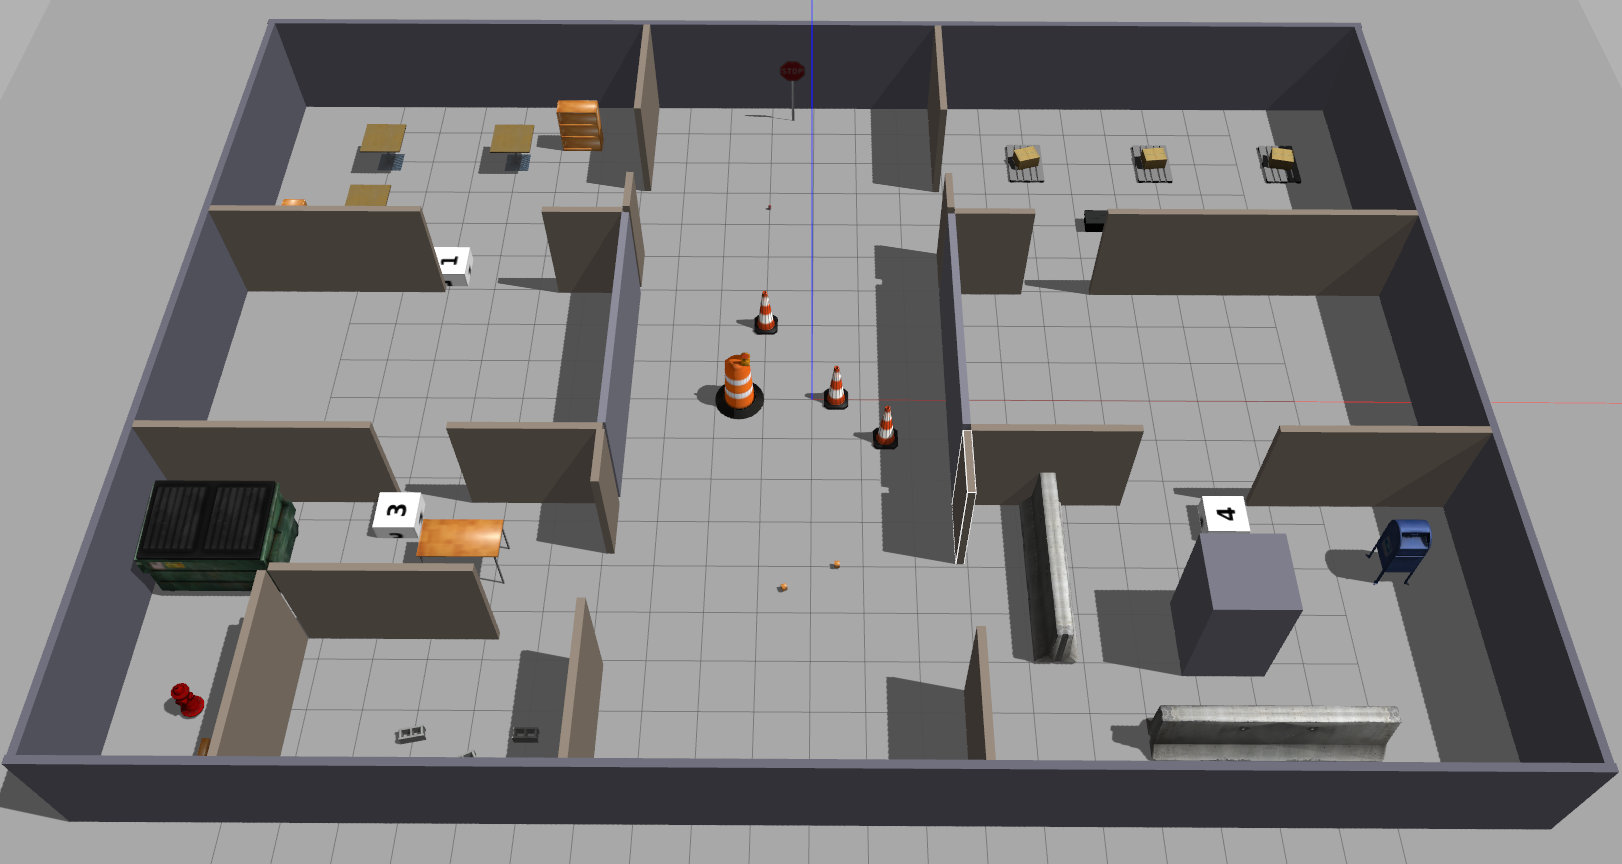
\includegraphics[width=0.9\linewidth]{figures/Chapter 5/Multi_robot_room.png}
    \caption{Multi-Robot Room: Swarm Coordination Testbed}
    \label{fig:multirobot_room}
\end{figure}

\section{Multi-Robot Swarm Architecture}
\label{sec:swarm_architecture}

Scaling from a single autonomous robot to a coordinated swarm introduces significant architectural challenges. Each robot must maintain its own independent perception, planning, and control pipeline while simultaneously participating in a shared communication network. The key enabler for this scalability is the systematic use of \textbf{namespaces}---a ROS 2 mechanism that prefixes all node names, topics, services, and TF frames with a unique identifier.

\subsection{Namespace-Based Scalability}

In ROS 2, namespaces provide logical isolation between robot instances. When a robot is launched with namespace \texttt{ausra\_1}, all its nodes and topics are automatically prefixed:

\begin{itemize}
    \item \texttt{/ausra\_1/scan} instead of \texttt{/scan}
    \item \texttt{/ausra\_1/cmd\_vel} instead of \texttt{/cmd\_vel}
    \item \texttt{/ausra\_1/odom} instead of \texttt{/odom}
    \item TF frames become \texttt{ausra\_1/base\_link}, \texttt{ausra\_1/odom}, etc.
\end{itemize}

This approach offers several critical advantages for swarm deployment:

\begin{enumerate}
    \item \textbf{Zero Code Modification:} The same Docker image, launch files, and configuration can be deployed to any number of robots by simply changing the namespace parameter
    \item \textbf{Topic Isolation:} Each robot's sensor data, control commands, and state estimates remain separate, preventing cross-contamination
    \item \textbf{TF Tree Independence:} Each robot maintains its own transform tree, avoiding the ``TF buffer collisions'' that occur when multiple robots publish to the same frame names
    \item \textbf{Selective Sharing:} Global topics (e.g., \texttt{/map}, \texttt{/swarm/status}) can remain outside namespaces for inter-robot coordination
\end{enumerate}

\begin{figure}[H]
    \centering
    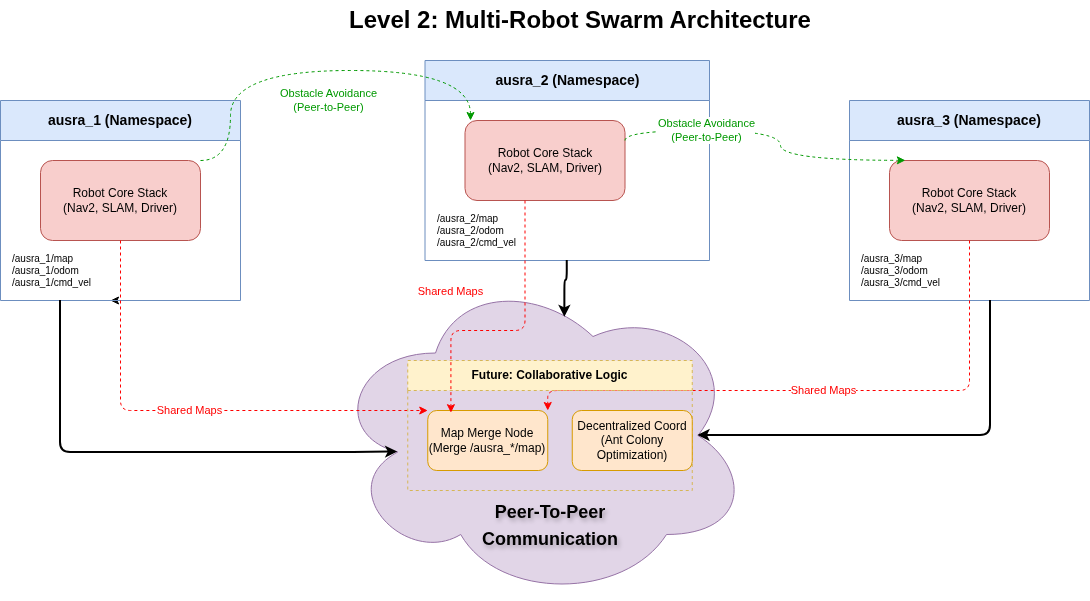
\includegraphics[width=1.0\linewidth]{figures/Chapter 5/Multi_robot_architecture.png}
    \caption{Level 2: Multi-Robot Swarm Architecture with Namespace Isolation}
    \label{fig:multi_robot_arch}
\end{figure}

\subsection{RQT Graph Analysis: Dual-Robot Operation}

Figure \ref{fig:rqt_namespace} presents the actual ROS 2 computation graph captured during simultaneous operation of two AUSRA robots (\texttt{ausra\_1} and \texttt{ausra\_2}) in Gazebo simulation. This visualization, generated using \texttt{rqt\_graph}, demonstrates the namespace isolation in practice.

\begin{figure}[H]
    \centering
    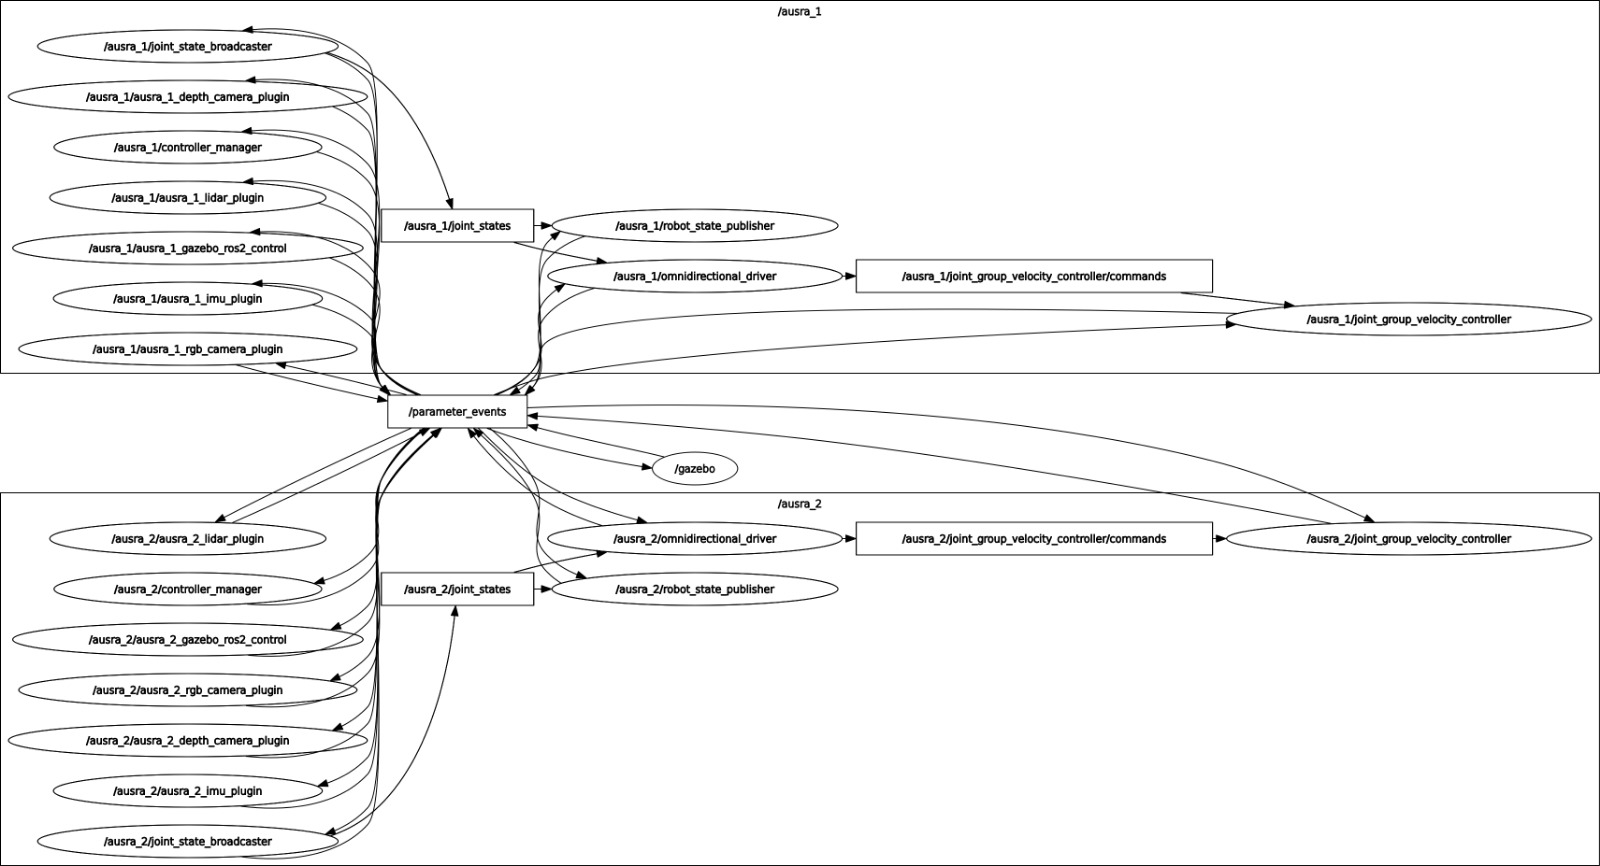
\includegraphics[width=1.0\linewidth]{figures/Chapter 5/Namespaces_of_2_robots.jpeg}
    \caption{RQT Graph: Dual-Robot Namespace Isolation During Simultaneous Operation}
    \label{fig:rqt_namespace}
\end{figure}

\subsubsection{Graph Structure Analysis}

The rqt\_graph reveals the complete node topology for both robots:

\paragraph{Per-Robot Node Set}
Each namespace contains an identical set of nodes:
\begin{itemize}
    \item \texttt{joint\_state\_broadcaster}: Publishes joint positions from Gazebo
    \item \texttt{robot\_state\_publisher}: Converts joint states to TF transforms
    \item \texttt{controller\_manager}: Manages ros2\_control lifecycle
    \item \texttt{omnidirectional\_driver}: Converts \texttt{cmd\_vel} to wheel commands
    \item \texttt{joint\_group\_velocity\_controller}: Executes wheel velocity commands
    \item Sensor plugins: \texttt{lidar\_plugin}, \texttt{imu\_plugin}, \texttt{depth\_camera\_plugin}, \texttt{rgb\_camera\_plugin}
\end{itemize}

\paragraph{Topic Flow Pattern}
The graph shows the data flow within each namespace:
\begin{enumerate}
    \item Sensor plugins publish to namespaced topics (e.g., \texttt{/ausra\_1/scan})
    \item \texttt{joint\_states} topic aggregates all joint positions
    \item \texttt{robot\_state\_publisher} broadcasts TF transforms
    \item \texttt{omnidirectional\_driver} subscribes to \texttt{cmd\_vel} and publishes to \texttt{joint\_group\_velocity\_controller/commands}
\end{enumerate}

\paragraph{Shared Resources}
Two elements remain outside namespaces:
\begin{itemize}
    \item \texttt{/gazebo}: The physics simulator node, shared by all robots
    \item \texttt{/parameter\_events}: ROS 2 system topic for parameter change notifications
\end{itemize}

\subsection{Docker-Based Swarm Deployment}

The namespace architecture integrates seamlessly with Docker containerization, enabling a ``build once, deploy everywhere'' strategy for swarm scaling.

\subsubsection{Deployment Architecture}

Each physical robot runs an identical Docker container with only one differentiating parameter:

\begin{verbatim}
# Robot 1
docker run --runtime nvidia --network host \
  -e ROBOT_NAMESPACE=ausra_1 \
  ausra_ros2:humble

# Robot 2
docker run --runtime nvidia --network host \
  -e ROBOT_NAMESPACE=ausra_2 \
  ausra_ros2:humble

# Robot N
docker run --runtime nvidia --network host \
  -e ROBOT_NAMESPACE=ausra_N \
  ausra_ros2:humble
\end{verbatim}

\subsubsection{Scalability Benefits}

This architecture provides significant operational advantages:

\begin{table}[H]
\centering
\caption{Docker + Namespace Scalability Benefits}
\label{tab:docker_scalability}
\begin{tabular}{|l|p{9cm}|}
\hline
\textbf{Benefit} & \textbf{Description} \\
\hline
Identical Images & Single Docker image for entire swarm; no per-robot customization \\
\hline
Rapid Deployment & New robots join swarm in seconds via container launch \\
\hline
Version Consistency & All robots run identical software versions, eliminating ``works on my robot'' issues \\
\hline
Easy Updates & Push new image to registry; all robots pull and restart \\
\hline
Failure Isolation & Container crash affects only one robot; others continue operating \\
\hline
Resource Management & Docker limits CPU/memory per robot, preventing runaway processes \\
\hline
\end{tabular}
\end{table}

\subsubsection{Launch File Integration}

The launch system automatically applies namespaces to all nodes:

\begin{verbatim}
# In launch file
namespace = LaunchConfiguration('robot_namespace')

Node(
    package='slam_toolbox',
    executable='async_slam_toolbox_node',
    namespace=namespace,
    parameters=[{'use_sim_time': True}],
    remappings=[('/tf', 'tf'), ('/tf_static', 'tf_static')]
)
\end{verbatim}

The \texttt{remappings} ensure TF topics remain global for multi-robot SLAM coordination while all other topics are namespaced.

\subsection{Swarm Communication Topology}

With namespace isolation established, robots communicate through two distinct channels:

\begin{enumerate}
    \item \textbf{Namespaced Topics:} Robot-specific data (sensor readings, local state)
    \item \textbf{Global Topics:} Swarm-level coordination (task allocation, shared map, inter-robot poses)
\end{enumerate}

\begin{table}[H]
\centering
\caption{Topic Namespace Strategy}
\label{tab:topic_namespace}
\begin{tabular}{|l|l|l|}
\hline
\textbf{Topic Type} & \textbf{Example} & \textbf{Namespace} \\
\hline
Sensor Data & \texttt{/ausra\_1/scan} & Per-robot \\
Odometry & \texttt{/ausra\_1/odom} & Per-robot \\
Control Commands & \texttt{/ausra\_1/cmd\_vel} & Per-robot \\
Robot Pose Broadcast & \texttt{/swarm/poses} & Global \\
Task Allocation & \texttt{/swarm/tasks} & Global \\
Merged Map & \texttt{/map} & Global \\
Emergency Stop & \texttt{/swarm/estop} & Global \\
\hline
\end{tabular}
\end{table}

\section{Communication Stack}
\label{sec:communication}

\subsection{DDS Middleware Configuration}

ROS 2 communication relies on the Data Distribution Service (DDS) middleware. For swarm operation, proper DDS configuration is critical:

\begin{itemize}
    \item \textbf{Discovery:} Automatic peer discovery via multicast (requires \texttt{network\_mode: host} in Docker)
    \item \textbf{Domain ID:} All swarm robots share the same \texttt{ROS\_DOMAIN\_ID} for mutual visibility
    \item \textbf{QoS Profiles:} Configured per-topic based on reliability requirements
\end{itemize}

\subsection{Quality of Service Configuration}

\begin{table}[H]
\centering
\caption{QoS Configuration by Topic Type}
\label{tab:qos_config}
\begin{tabular}{|l|c|c|c|}
\hline
\textbf{Topic} & \textbf{Reliability} & \textbf{Durability} & \textbf{History} \\
\hline
/scan, /imu & Best Effort & Volatile & Keep Last (5) \\
/cmd\_vel & Reliable & Volatile & Keep Last (1) \\
/map & Reliable & Transient Local & Keep Last (1) \\
/swarm/tasks & Reliable & Transient Local & Keep All \\
/tf & Reliable & Volatile & Keep Last (100) \\
\hline
\end{tabular}
\end{table}

\subsection{Inter-Robot Communication}

Communication between robots is achieved through the shared DDS network:

\begin{itemize}
    \item \textbf{Transport:} WiFi-based UDP/TCP with automatic failover
    \item \textbf{Middleware:} Cyclone DDS (default for ROS 2 Humble) with tuned buffer sizes
    \item \textbf{Message Types:}
    \begin{itemize}
        \item \texttt{geometry\_msgs/PoseStamped}: Robot pose broadcasts at 10 Hz
        \item \texttt{nav\_msgs/OccupancyGrid}: Map sharing for collaborative SLAM
        \item \texttt{std\_msgs/String}: Task allocation and status messages
    \end{itemize}
\end{itemize}

% Add your detailed content here...

\section{The Autonomous System}
\label{sec:autonomous_system}

\subsection{Sensor Fusion and Localization}
\label{subsec:localization}

Accurate state estimation requires fusing multiple sensors with complementary characteristics. Wheel encoders provide good short-term position estimates but suffer from cumulative drift. The IMU provides excellent short-term orientation but drifts over longer periods. The Extended Kalman Filter (EKF) produces optimal estimates more accurate than any single sensor.

\subsubsection{Extended Kalman Filter Architecture}

The \texttt{robot\_localization} package implements the EKF for sensor fusion, configured via \texttt{ekf.yaml}:

\paragraph{State Vector}
\begin{equation}
\mathbf{x} = [x, y, z, \phi, \theta, \psi, \dot{x}, \dot{y}, \dot{z}, \dot{\phi}, \dot{\theta}, \dot{\psi}, \ddot{x}, \ddot{y}, \ddot{z}]^T
\label{eq:state_vector}
\end{equation}

\paragraph{Sensor Configuration}
\begin{itemize}
    \item \textbf{Wheel Odometry (50 Hz):} Provides $x$, $y$ position and $\psi$ (yaw) orientation
    \item \textbf{IMU (100 Hz):} Provides angular velocity ($\dot{\phi}, \dot{\theta}, \dot{\psi}$) and linear acceleration ($\ddot{x}, \ddot{y}, \ddot{z}$)
    \item \textbf{Visual Odometry (10--30 Hz):} Validates wheel data during slip conditions
\end{itemize}

\paragraph{Covariance Tuning}
Process noise and sensor covariances critically affect filter performance:
\begin{itemize}
    \item \textbf{IMU Angular Velocity:} 0.001 (rad/s)$^2$ diagonal covariance
    \item \textbf{IMU Linear Acceleration:} 0.01 (m/s$^2$)$^2$ diagonal covariance
    \item \textbf{Wheel Odometry Position:} Values tuned based on encoder resolution and wheel slip characteristics
\end{itemize}

\subsubsection{ROS 2 IMU Driver Implementation}

The \texttt{imu\_esp32\_bridge} package provides the bridge between hardware and ROS 2:

\paragraph{Topics Published}
\begin{itemize}
    \item \texttt{/imu/data\_raw}: Combined accelerometer/gyroscope data (\texttt{sensor\_msgs/Imu})
    \item \texttt{/imu/mag}: Magnetometer data (\texttt{sensor\_msgs/MagneticField})
\end{itemize}

\paragraph{Unit Conversions}
\begin{itemize}
    \item Accelerometer: $g \rightarrow$ m/s$^2$ (multiply by 9.81)
    \item Gyroscope: °/s $\rightarrow$ rad/s (multiply by $\pi$/180)
    \item Magnetometer: $\mu$T $\rightarrow$ T (multiply by $10^{-6}$)
\end{itemize}

\begin{figure}[H]
    \centering
    \begin{subfigure}[b]{0.45\textwidth}
        \centering
        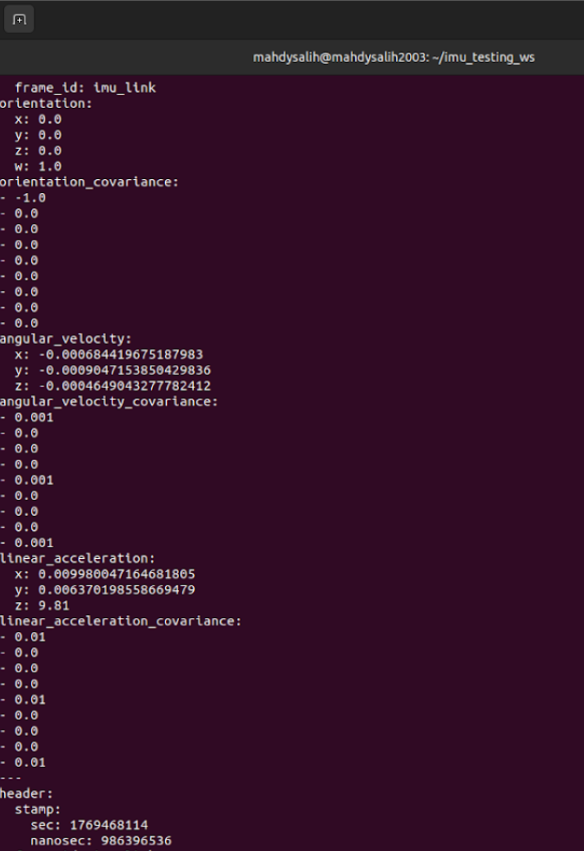
\includegraphics[width=\linewidth]{figures/Chapter 5/IMU_terminal.png}
        \caption{IMU Data Stream}
        \label{fig:imu_terminal}
    \end{subfigure}
    \hfill
    \begin{subfigure}[b]{0.45\textwidth}
        \centering
        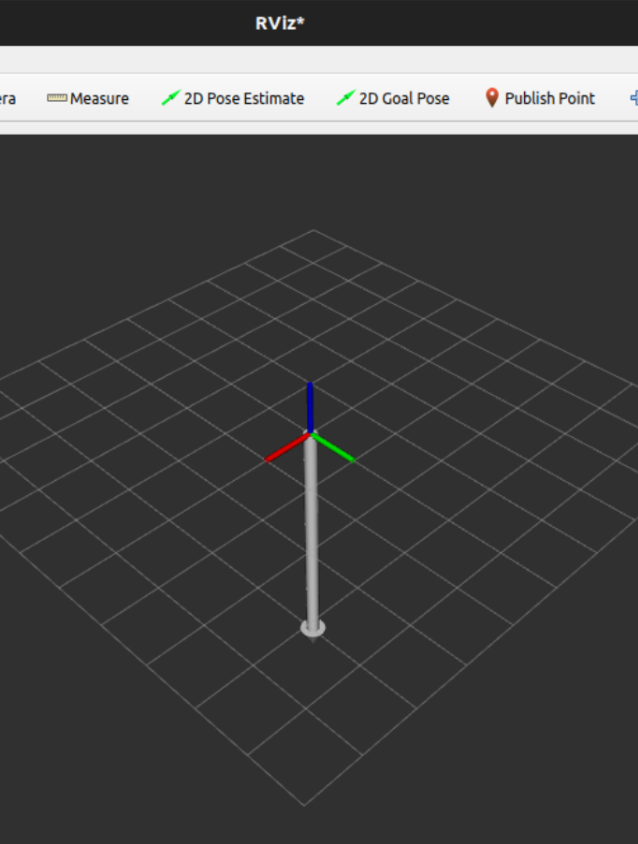
\includegraphics[width=\linewidth]{figures/Chapter 5/IMU_rviz.png}
        \caption{IMU Visualization in RViz2}
        \label{fig:imu_rviz}
    \end{subfigure}
    \caption{IMU Data Acquisition and Visualization}
    \label{fig:imu_data}
\end{figure}

\subsubsection{Visualization and Validation}

\begin{figure}[H]
    \centering
    \begin{subfigure}[b]{0.45\textwidth}
        \centering
        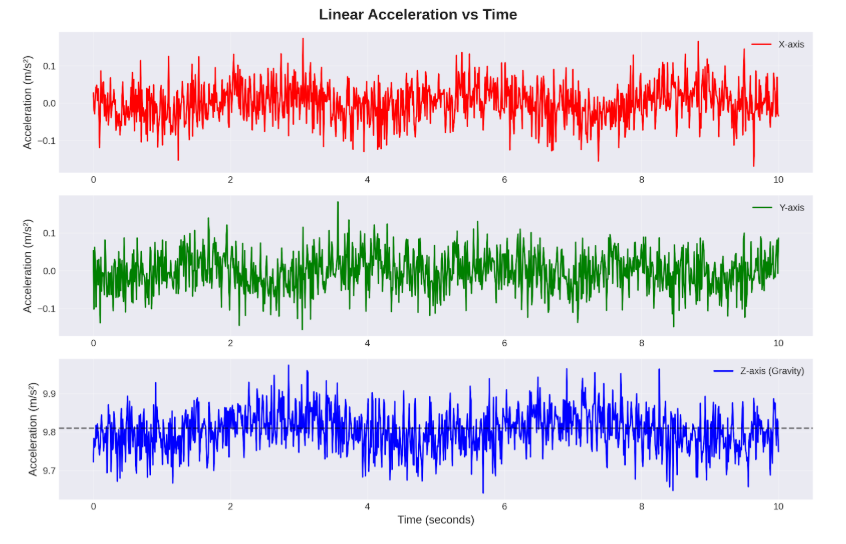
\includegraphics[width=\linewidth]{figures/Chapter 5/Linear_acc.png}
        \caption{Linear Acceleration (Z-axis showing gravity)}
        \label{fig:linear_acc}
    \end{subfigure}
    \hfill
    \begin{subfigure}[b]{0.45\textwidth}
        \centering
        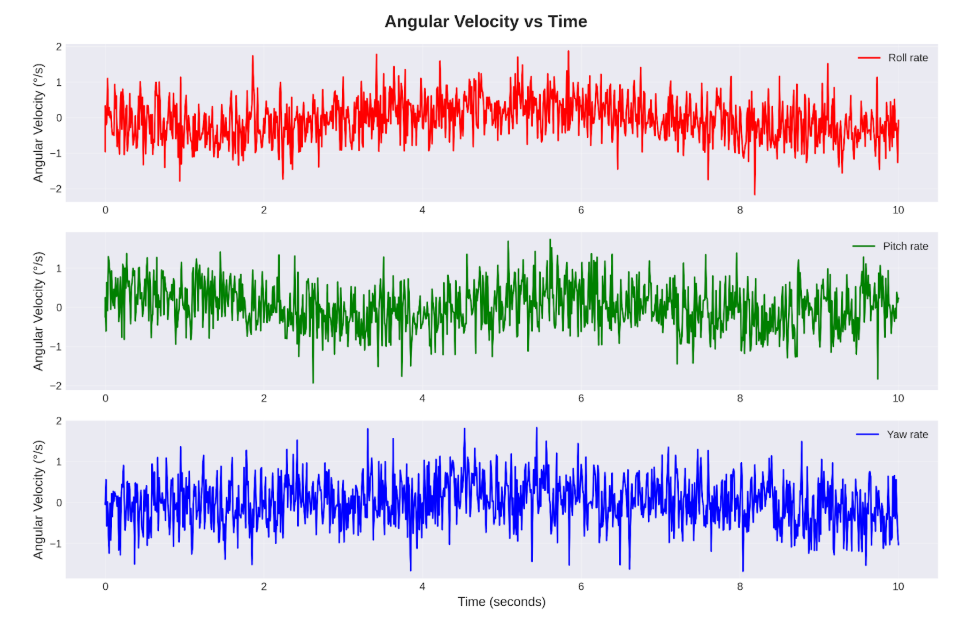
\includegraphics[width=\linewidth]{figures/Chapter 5/Angular_vel.png}
        \caption{Angular Velocity During Rotation}
        \label{fig:angular_vel}
    \end{subfigure}
    \caption{IMU Sensor Measurements}
    \label{fig:imu_measurements}
\end{figure}

Key observations from visualization analysis:
\begin{itemize}
    \item Noise characteristics validate EKF covariance parameters
    \item Absence of systematic drift confirms calibration effectiveness
    \item Clear gravity measurement ($\approx$9.81 m/s$^2$ on Z-axis) demonstrates adequate sensor performance
\end{itemize}

\subsubsection{Direct Jetson Integration}

For production deployment, direct Jetson Orin Nano integration eliminates the ESP32 bridge:
\begin{itemize}
    \item \textbf{Latency Reduction:} 35--55 ms improvement (from 58 ms to 14 ms end-to-end)
    \item \textbf{Simplified Architecture:} Eliminates USB serial communication overhead
    \item \textbf{I2C Connection:} Pins 3 (SDA) and 5 (SCL) on Jetson 40-pin header at 400 kHz
\end{itemize}

\subsubsection{SLAM Integration}

\paragraph{The Navigation Problem}
Autonomous navigation in unknown environments requires solving three interdependent problems:
\begin{enumerate}
    \item \textbf{Localization:} Continuous pose estimation relative to a reference frame
    \item \textbf{Mapping:} Constructing an environment representation for obstacle identification
    \item \textbf{Path Planning:} Calculating safe, efficient trajectories dependent on both localization and mapping
\end{enumerate}

\paragraph{Challenges in Unstructured Environments}
Real-world environments present unique challenges:
\begin{itemize}
    \item \textbf{Unstructured Geometry:} Irregular shapes and unexpected obstacles
    \item \textbf{GPS-Denied Operation:} Indoor and underground areas require internal sensors for localization
    \item \textbf{Kinematic Instability:} Wheel slippage invalidates dead reckoning
\end{itemize}

\paragraph{SLAM: Simultaneous Localization and Mapping}
SLAM addresses the fundamental interdependence: accurate mapping requires known position, while localization requires a reference map. The algorithm constructs a map while determining the robot's location within it.

SLAM is formulated as a probabilistic problem, estimating the posterior probability distribution of the robot's path and map given noisy sensor data.

\subsection{Mapping with slam\_toolbox}
\label{subsec:slam_toolbox}

The \texttt{slam\_toolbox} package is a graph-based SLAM framework for ROS 2, selected for its robust loop closure, efficient optimization, and tight ROS 2 integration. Alternative approaches such as GMapping \cite{grisetti2007improved} and Google Cartographer \cite{hess2016cartographer} were evaluated but ultimately \texttt{slam\_toolbox} was chosen for its superior performance in dynamic environments.

\subsubsection{Algorithm Selection}

\begin{table}[H]
\centering
\caption{SLAM Algorithm Selection Matrix}
\label{tab:slam_selection}
\begin{tabular}{|l|c|c|c|c|c|c|c|}
\hline
\textbf{Criteria} & \textbf{Weight} & \multicolumn{2}{c|}{\textbf{slam\_toolbox}} & \multicolumn{2}{c|}{\textbf{Gmapping}} & \multicolumn{2}{c|}{\textbf{Hector}} \\
\cline{3-8}
 & & Rate & Score & Rate & Score & Rate & Score \\
\hline
Sensor Fusion & 5 & 4 & 20 & 5 & 25 & 0 & 0 \\
\hline
Loop Closure & 5 & 5 & 25 & 1 & 5 & 0 & 0 \\
\hline
Indoor Suitability & 5 & 5 & 25 & 4 & 20 & 4 & 20 \\
\hline
Map Sharpness & 4 & 4 & 16 & 3 & 12 & 5 & 20 \\
\hline
ROS 2 Maturity & 4 & 5 & 20 & 1 & 4 & 2 & 8 \\
\hline
Computational Cost & 3 & 4 & 12 & 4 & 12 & 5 & 15 \\
\hline
\textbf{Final Score} & & & \textbf{118} & & \textbf{78} & & \textbf{63} \\
\hline
\end{tabular}
\end{table}

\subsubsection{System Architecture}

\begin{figure}[H]
    \centering
    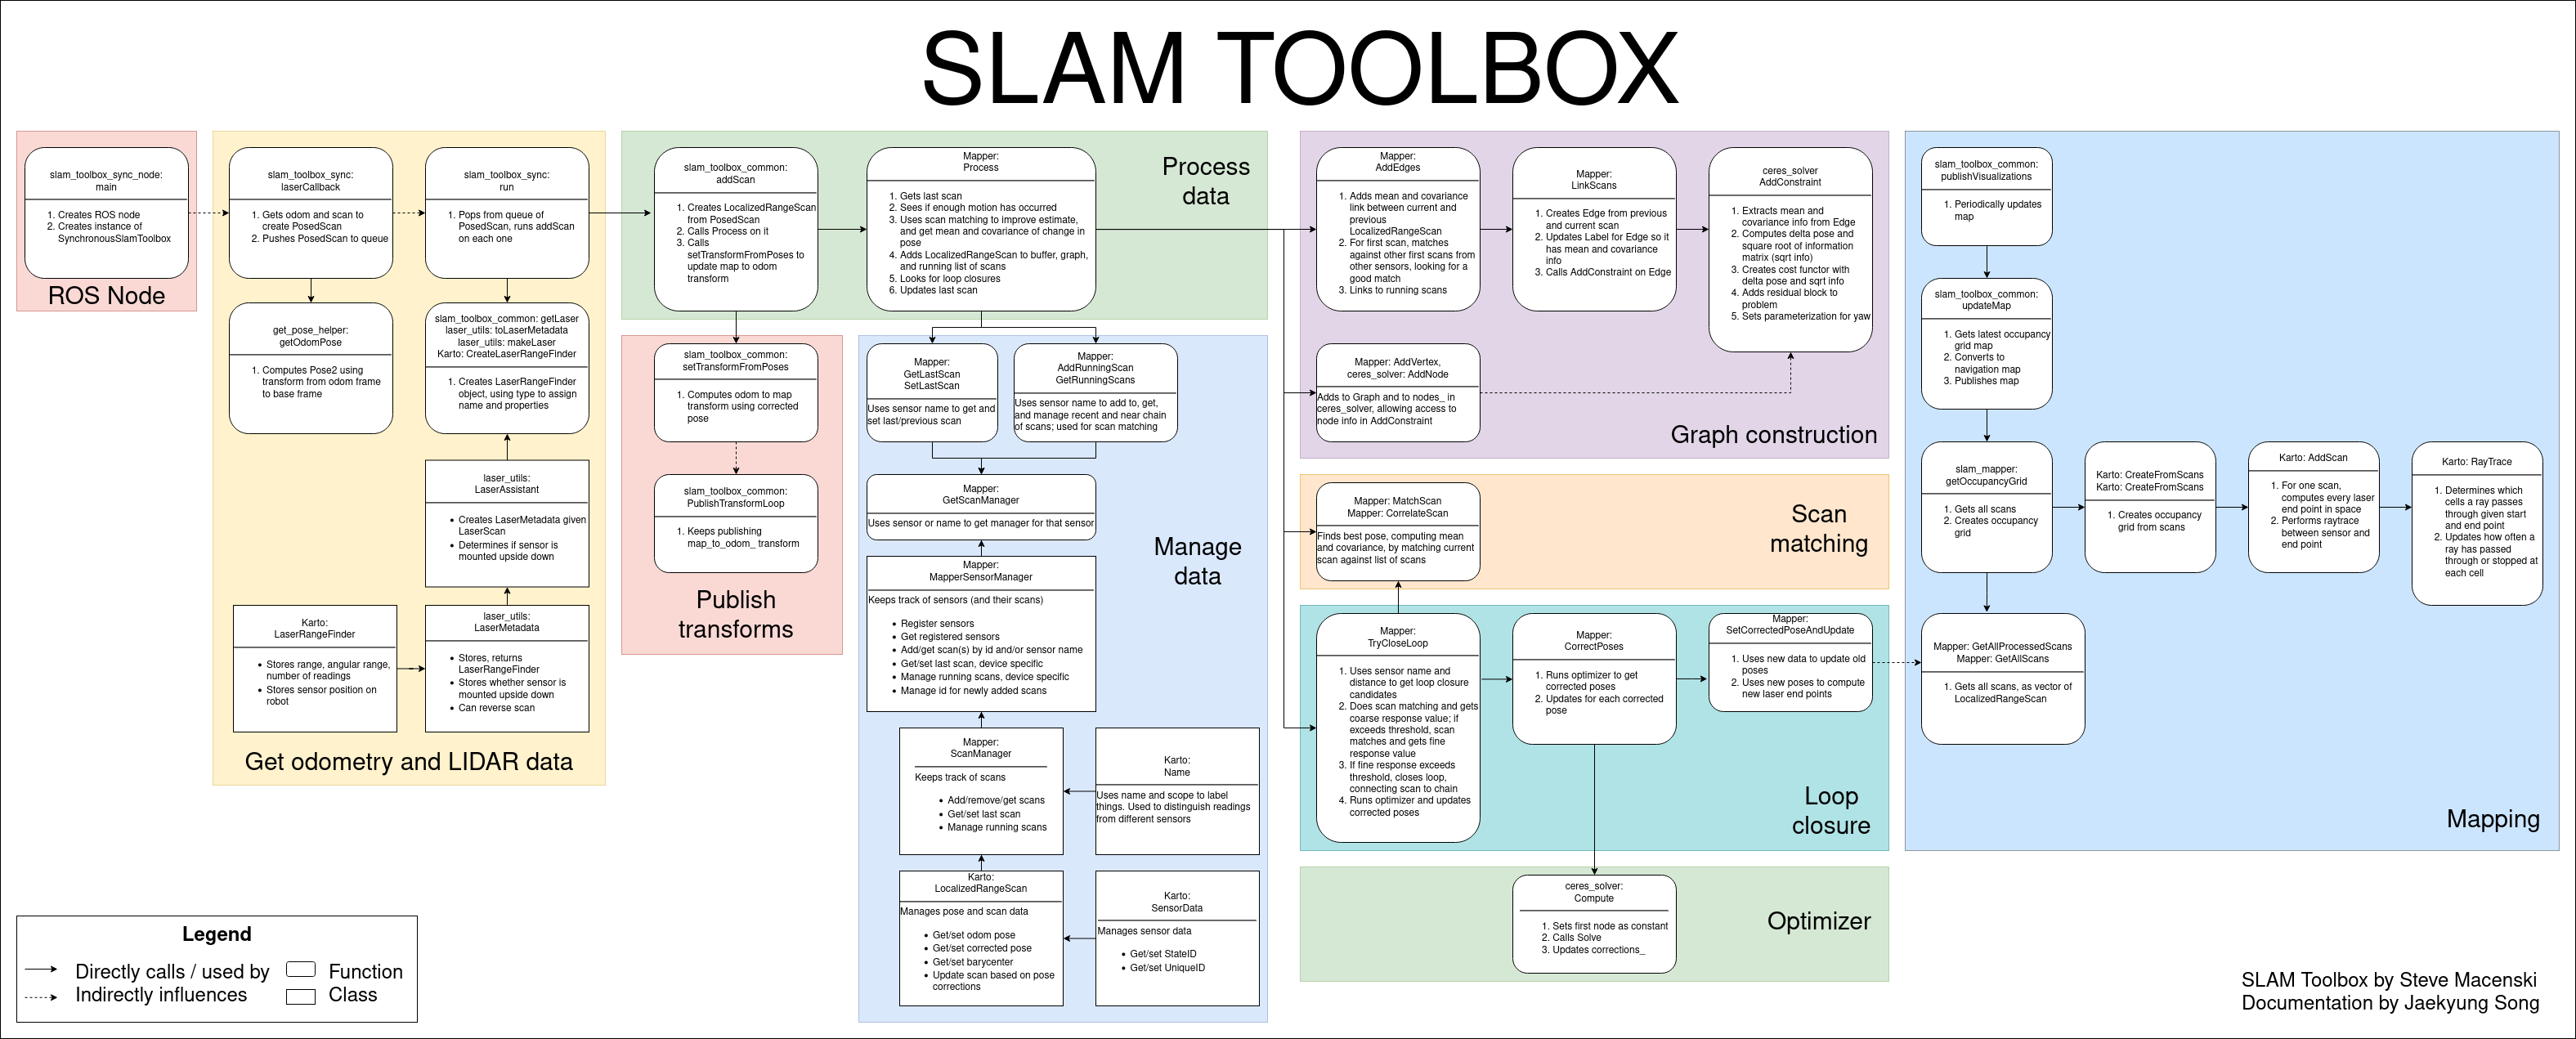
\includegraphics[width=0.85\linewidth]{figures/Chapter 5/slam_toolbox_sync.png}
    \caption{slam\_toolbox System Architecture}
    \label{fig:slam_toolbox_arch}
\end{figure}

The pipeline consists of:
\begin{enumerate}
    \item \textbf{Sensor Data Acquisition:} LiDAR scans and odometry input
    \item \textbf{Pose Graph Construction:} Nodes represent poses, edges encode constraints
    \item \textbf{Scan Matching:} Aligns consecutive scans for relative motion
    \item \textbf{Loop Closure Detection:} Identifies previously visited locations
    \item \textbf{Graph Optimization:} Minimizes constraint errors using Ceres Solver
    \item \textbf{Map Generation:} Outputs occupancy grid
\end{enumerate}

\paragraph{Pose Graph Representation}
Each node represents robot pose $\mathbf{x}_i = [x_i, y_i, \theta_i]^T$. Edges encode relative measurements:
\begin{equation}
\mathbf{z}_{ij} = \mathbf{x}_j \ominus \mathbf{x}_i
\label{eq:relative_pose}
\end{equation}

\paragraph{Maximum Likelihood Formulation}
The optimization minimizes:
\begin{equation}
\mathbf{X}^* = \arg\min_{\mathbf{X}} \sum_{(i,j) \in E} \|\mathbf{z}_{ij} - h(\mathbf{x}_i, \mathbf{x}_j)\|^2_{\Omega_{ij}}
\label{eq:slam_optimization}
\end{equation}
where $\Omega_{ij}$ is the information matrix weighting constraint confidence.

\subsubsection{ROS 2 Topics and Frames}

\begin{table}[H]
\centering
\caption{slam\_toolbox ROS 2 Interface}
\label{tab:slam_topics}
\begin{tabular}{|l|l|l|}
\hline
\textbf{Topic} & \textbf{Type} & \textbf{Description} \\
\hline
/scan & sensor\_msgs/LaserScan & LiDAR input \\
/odom & nav\_msgs/Odometry & Wheel odometry \\
/map & nav\_msgs/OccupancyGrid & Output map \\
/tf & tf2\_msgs/TFMessage & Coordinate transforms \\
\hline
\end{tabular}
\end{table}

Transform chain: \texttt{map} $\rightarrow$ \texttt{odom} (from slam\_toolbox) $\rightarrow$ \texttt{base\_link} (from EKF).

\subsubsection{Parameter Tuning Strategy}

Parameters were tuned to address specific mapping artifacts:

\paragraph{Wall Thickness Reduction}
Excessive wall thickness results from pose estimation errors. Scan matching precision was increased, and occupancy probability thresholds were tuned.

\begin{figure}[H]
    \centering
    \begin{subfigure}[b]{0.45\textwidth}
        \centering
        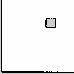
\includegraphics[width=\linewidth]{figures/Chapter 5/wall_thickness_before.png}
        \caption{Before Tuning}
        \label{fig:wall_thick_before}
    \end{subfigure}
    \hfill
    \begin{subfigure}[b]{0.45\textwidth}
        \centering
        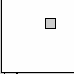
\includegraphics[width=\linewidth]{figures/Chapter 5/wall_thickness_after.png}
        \caption{After Tuning}
        \label{fig:wall_thick_after}
    \end{subfigure}
    \caption{Wall Thickness Optimization}
    \label{fig:wall_thickness}
\end{figure}

\paragraph{Corner Preservation}
Wall discontinuities occur with insufficient scan matching confidence. Angle variance penalties were increased to prevent corner deformation.

\begin{figure}[H]
    \centering
    \begin{subfigure}[b]{0.45\textwidth}
        \centering
        
\includegraphics[width=\linewidth]{figures/Chapter 5/wall_discontinuity_before.png}
        \caption{Before Tuning}
        \label{fig:corner_before}
    \end{subfigure}
    \hfill
    \begin{subfigure}[b]{0.45\textwidth}
        \centering
        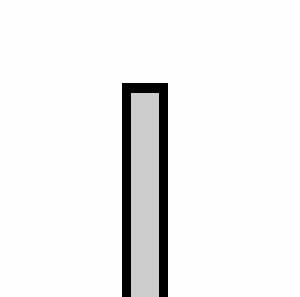
\includegraphics[width=\linewidth]{figures/Chapter 5/wall_discontinuity_after.png}
        \caption{After Tuning}
        \label{fig:corner_after}
    \end{subfigure}
    \caption{Corner Preservation Optimization}
    \label{fig:corner_preservation}
\end{figure}

\subsubsection{Experimental Results}

\begin{figure}[H]
    \centering
    \begin{subfigure}[b]{0.45\textwidth}
        \centering
        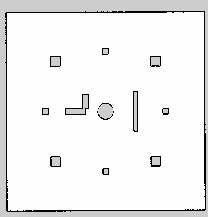
\includegraphics[width=\linewidth]{figures/Chapter 5/room1_map_trial3.png}
        \caption{Single Room Environment}
        \label{fig:room1_map}
    \end{subfigure}
    \hfill
    \begin{subfigure}[b]{0.45\textwidth}
        \centering
        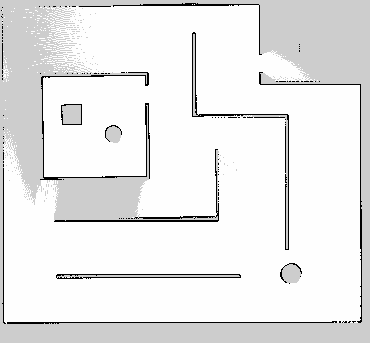
\includegraphics[width=\linewidth]{figures/Chapter 5/room2_map_trial1.png}
        \caption{Corridor Environment}
        \label{fig:room2_map}
    \end{subfigure}
    \caption{slam\_toolbox Mapping Results}
    \label{fig:slam_results}
\end{figure}

\begin{figure}[H]
    \centering
    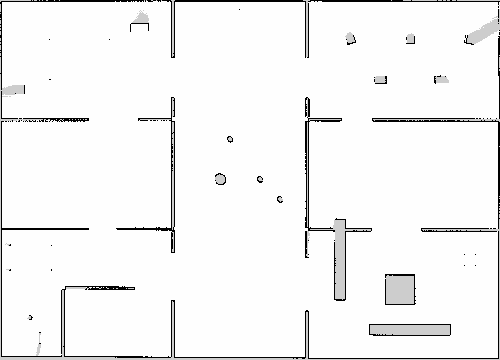
\includegraphics[width=0.7\linewidth]{figures/Chapter 5/multirobot_room_map.png}
    \caption{Multi-Room Environment Mapping}
    \label{fig:multiroom_map}
\end{figure}

The generated maps exhibit clear wall boundaries, consistent room shapes, and minimal drift after loop closure.

\subsection{Google Cartographer SLAM}
\label{subsec:cartographer}

Google Cartographer was evaluated as an alternative graph-based SLAM framework with advanced loop closure capabilities.

\subsubsection{Algorithm Selection}

\begin{table}[H]
\centering
\caption{Cartographer Selection Matrix}
\label{tab:cartographer_selection}
\begin{tabular}{|l|c|c|c|c|c|c|c|}
\hline
\textbf{Criteria} & \textbf{Weight} & \multicolumn{2}{c|}{\textbf{Cartographer}} & \multicolumn{2}{c|}{\textbf{Gmapping}} & \multicolumn{2}{c|}{\textbf{Hector}} \\
\cline{3-8}
 & & Rate & Score & Rate & Score & Rate & Score \\
\hline
Sensor Fusion & 5 & 5 & 25 & 5 & 25 & 0 & 0 \\
\hline
Loop Closure & 5 & 5 & 25 & 1 & 5 & 0 & 0 \\
\hline
Indoor Suitability & 5 & 5 & 25 & 4 & 20 & 4 & 20 \\
\hline
Map Sharpness & 4 & 5 & 20 & 3 & 12 & 5 & 20 \\
\hline
ROS 2 Maturity & 4 & 5 & 20 & 1 & 4 & 2 & 8 \\
\hline
Computational Cost & 3 & 3 & 9 & 4 & 12 & 5 & 15 \\
\hline
\textbf{Final Score} & & & \textbf{124} & & \textbf{78} & & \textbf{63} \\
\hline
\end{tabular}
\end{table}

\subsubsection{System Architecture}

\begin{figure}[H]
    \centering
    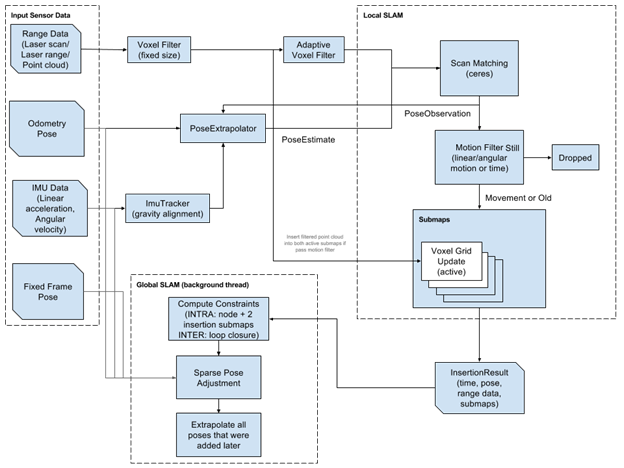
\includegraphics[width=0.9\linewidth]{figures/Chapter 5/cartographer_architecture.png}
    \caption{Google Cartographer Architecture}
    \label{fig:cartographer_arch}
\end{figure}

Cartographer operates with two asynchronous subsystems:
\begin{itemize}
    \item \textbf{Local SLAM (Front-End):} Processes sensor data for immediate trajectory estimation using submaps
    \item \textbf{Global SLAM (Back-End):} Optimizes the pose graph to correct long-term drift
\end{itemize}

\paragraph{Input Data}
\begin{itemize}
    \item \textbf{Range Data:} 2D LiDAR scans
    \item \textbf{Odometry:} Wheel encoder data ($v_x$, $v_y$, $\omega$)
    \item \textbf{IMU:} Angular velocity and linear acceleration for gravity alignment
\end{itemize}

\subsubsection{Local SLAM: Trajectory Builder}

\paragraph{Probability Grids}
Unlike binary maps, Cartographer uses probability grids where each cell stores obstruction likelihood. Laser hits increase probability; passes decrease it.

\paragraph{Ceres Scan Matching}
The solver minimizes:
\begin{equation}
J(\xi) = \underbrace{\sum_{k=1}^{K} (1 - M_{smooth}(T_{\xi} h_k))^2}_{\text{Scan Match Cost}} + \underbrace{\lambda_t \|T_{\xi} - \xi_{odom}\|^2}_{\text{Translation Penalty}} + \underbrace{\lambda_r \|\theta_{\xi} - \theta_{odom}\|^2}_{\text{Rotation Penalty}}
\label{eq:ceres_cost}
\end{equation}
where $M_{smooth}$ is the interpolated map probability, and $\lambda_t$, $\lambda_r$ are trust weights.

\subsubsection{Global SLAM: Pose Graph Optimization}

\paragraph{Loop Closure via Branch-and-Bound}
Cartographer uses Branch-and-Bound to efficiently search for loop closures, discarding regions where the best possible match score is below threshold.

\paragraph{Sparse Pose Adjustment}
The optimizer minimizes total error energy:
\begin{equation}
\arg\min \sum_{ij} \mathbf{e}_{ij}^T \Omega_{ij} \mathbf{e}_{ij}
\label{eq:spa}
\end{equation}
where $\mathbf{e}_{ij}$ is the error between measured and estimated relative poses.

\subsubsection{Error Diagnosis and Tuning}

\paragraph{Odometry Drift Correction}

\begin{figure}[H]
    \centering
    \begin{subfigure}[b]{0.45\textwidth}
        \centering
        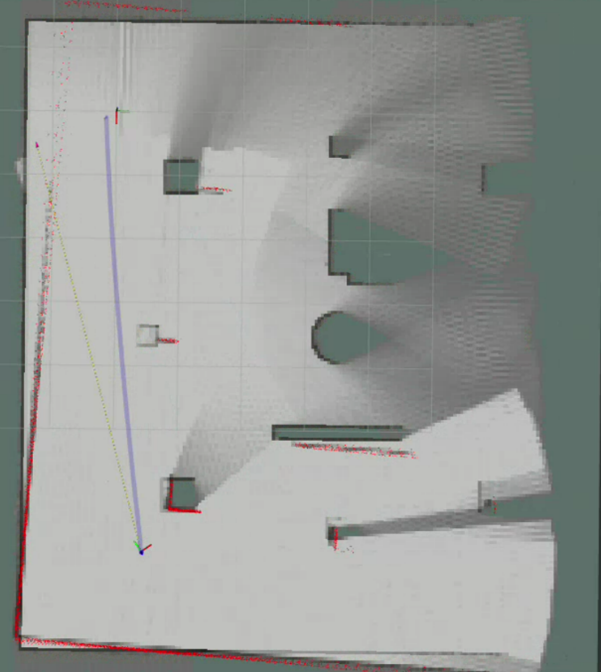
\includegraphics[width=\linewidth]{figures/Chapter 5/initial_odom_drift.png}
        \caption{Initial Drift}
        \label{fig:odom_drift}
    \end{subfigure}
    \hfill
    \begin{subfigure}[b]{0.45\textwidth}
        \centering
        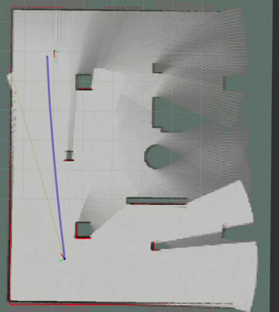
\includegraphics[width=\linewidth]{figures/Chapter 5/snap_correction.png}
        \caption{After Global Correction}
        \label{fig:snap_correction}
    \end{subfigure}
    \caption{Odometry Drift and Correction}
    \label{fig:drift_correction}
\end{figure}

\paragraph{Lateral Slip Compensation}
Omni-wheels cause lateral slip, producing ``ghosting'' artifacts. The Real-Time Correlative Scan Matcher was enabled with a 0.1m linear and 40° angular search window.

\begin{figure}[H]
    \centering
    \begin{subfigure}[b]{0.45\textwidth}
        \centering
        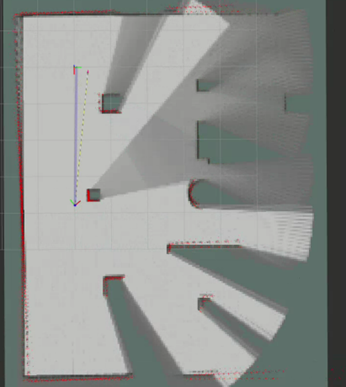
\includegraphics[width=\linewidth]{figures/Chapter 5/ghosting_problem.png}
        \caption{Ghosting Artifact}
        \label{fig:ghosting}
    \end{subfigure}
    \hfill
    \begin{subfigure}[b]{0.45\textwidth}
        \centering
        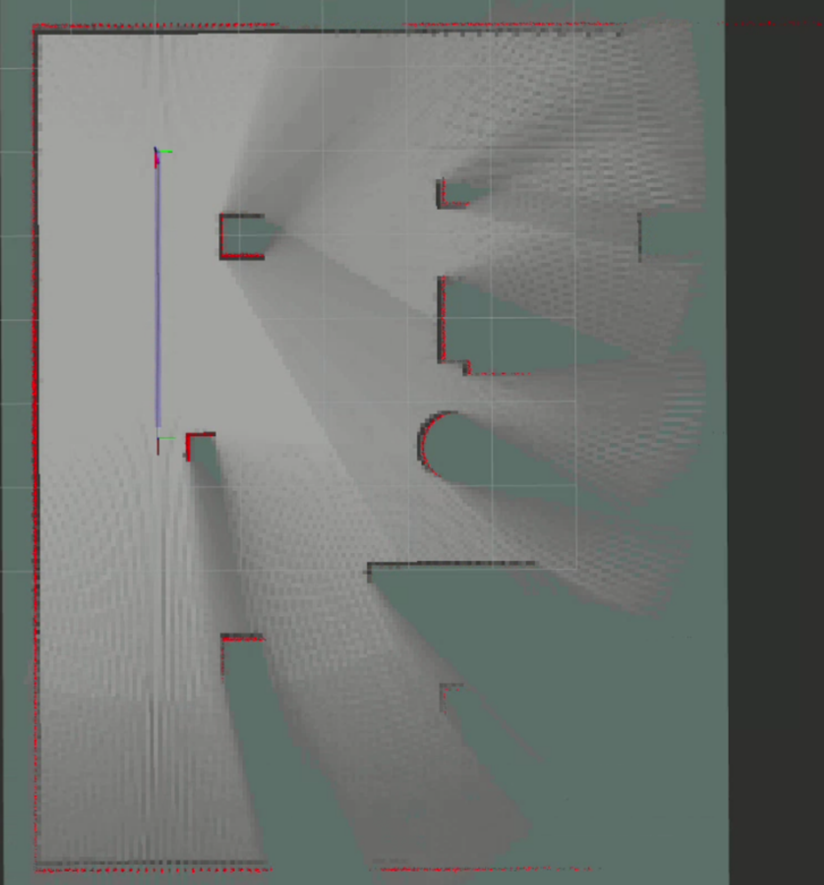
\includegraphics[width=\linewidth]{figures/Chapter 5/solved_ghosting.png}
        \caption{After Tuning}
        \label{fig:solved_ghosting}
    \end{subfigure}
    \caption{Lateral Slip Artifact Correction}
    \label{fig:ghosting_fix}
\end{figure}

\subsubsection{Final Configuration Parameters}

Key tuning parameters:
\begin{itemize}
    \item \textbf{Correlative Scan Matcher:} Enabled with 0.1m/40° search window
    \item \textbf{Ceres Weights:} Occupied space: 20, Translation: 10, Rotation: 40
    \item \textbf{Submaps:} 35 scans per submap for stability
    \item \textbf{Miss Probability:} 0.49 (conservative erasing)
    \item \textbf{Optimization Frequency:} Every 20 nodes
\end{itemize}

\subsubsection{Validation Results}

\begin{figure}[H]
    \centering
    \begin{subfigure}[b]{0.45\textwidth}
        \centering
        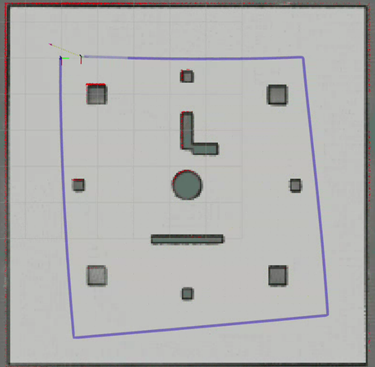
\includegraphics[width=\linewidth]{figures/Chapter 5/loop_closure_before.png}
        \caption{Before Loop Closure}
        \label{fig:loop_before}
    \end{subfigure}
    \hfill
    \begin{subfigure}[b]{0.45\textwidth}
        \centering
        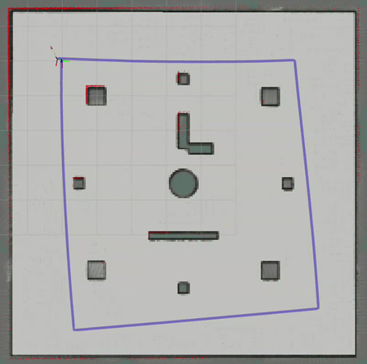
\includegraphics[width=\linewidth]{figures/Chapter 5/loop_closure_after.png}
        \caption{After Loop Closure}
        \label{fig:loop_after}
    \end{subfigure}
    \caption{Loop Closure Correction}
    \label{fig:loop_closure_results}
\end{figure}

\begin{figure}[H]
    \centering
    \begin{subfigure}[b]{0.45\textwidth}
        \centering
        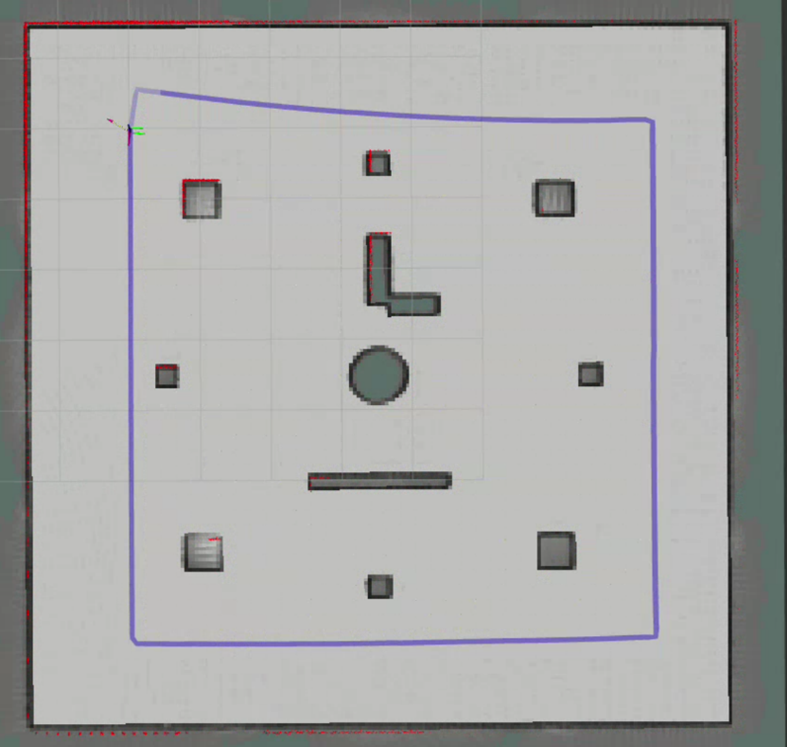
\includegraphics[width=\linewidth]{figures/Chapter 5/final tuned map.png}
        \caption{Tuned Navigation Map}
        \label{fig:final_map}
    \end{subfigure}
    \hfill
    \begin{subfigure}[b]{0.45\textwidth}
        \centering
        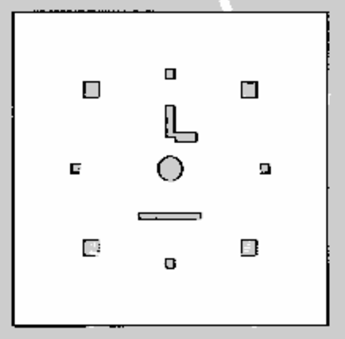
\includegraphics[width=\linewidth]{figures/Chapter 5/final_occupancy_grid_map.png}
        \caption{Final Occupancy Grid}
        \label{fig:final_grid}
    \end{subfigure}
    \caption{Cartographer Final Mapping Results}
    \label{fig:cartographer_results}
\end{figure}

\subsection{SLAM Framework Selection}
\label{subsec:slam_selection}

Both frameworks were evaluated under identical conditions. While Cartographer achieves high accuracy, it exhibited increased computational demand during loop closure and sensitivity to odometry noise and parameter tuning.

\texttt{slam\_toolbox} consistently produced maps with improved structural clarity, reduced wall thickening, and fewer alignment artifacts, indicating more effective scan-to-map alignment in the presence of sensor noise.

Based on the evaluation, \textbf{slam\_toolbox} was selected as the primary SLAM solution for:
\begin{itemize}
    \item \textbf{Map Quality:} Superior structural clarity
    \item \textbf{Computational Efficiency:} Lower resource requirements
    \item \textbf{Odometry Drift Correction:} Better handling of omni-directional kinematics
\end{itemize}

\subsection{SLAM Limitations and Future Work}
\label{subsec:slam_limitations}

\subsubsection{Current Limitations}
\begin{itemize}
    \item \textbf{Dynamic Obstacles:} Static occupancy grid assumption---moving objects cause mapping errors
    \item \textbf{Odometry Dependence:} Poor odometry quality degrades loop closure performance
    \item \textbf{Featureless Environments:} LiDAR-based SLAM struggles without geometric features
\end{itemize}

\subsubsection{Future Improvements}

\paragraph{Semantic SLAM}
Integrates deep learning-based perception to identify and classify objects, enabling human-like reasoning and improved navigation in dynamic environments.

\paragraph{Collaborative Mapping}
Extends SLAM to multi-robot systems where agents share map fragments, enabling faster exploration, improved completeness, and increased robustness against localization failures. Inter-robot loop closures significantly reduce accumulated drift across the swarm.

% Add your detailed content here...

\subsection{Planning}
\label{subsec:planning}

The navigation stack is built on Nav2, highly tuned for an omnidirectional robot.

\subsubsection{Global Planning (SmacPlanner A*)}

The \texttt{SmacPlanner2D} provides efficient grid-based A* planning:
\begin{itemize}
    \item \textbf{Optimization:} Handles large costmaps (up to $100m \times 100m$) with up to 1,000,000 iterations
    \item \textbf{Cost Penalty:} High \texttt{cost\_travel\_multiplier} (50.0) acts as a ``soft obstacle'' repulsor, forcing the robot to prefer safer paths through open spaces
    \item \textbf{Unknown Space:} \texttt{allow\_unknown: true} enables planning through unexplored areas for exploration tasks
\end{itemize}

\subsubsection{Local Control (DWB Holonomic)}

The local trajectory generation uses the Dynamic Window Approach (DWB) Local Planner \cite{fox1997dynamic}, configured for holonomic motion:
\begin{itemize}
    \item \textbf{Holonomic Sampling:} Samples velocities in both $v_x$ (forward/back) and $v_y$ (left/right) directions using a $15 \times 15$ sample grid
    \item \textbf{Twirling Critic:} High weight (10.0) penalizes unnecessary rotation, enabling the robot to strafe while maintaining sensor orientation
    \item \textbf{Obstacle Footprint:} Highest priority (Scale 100.0) for collision avoidance, ensuring immediate halt if trajectory intersects costmap footprint
\end{itemize}

See Appendix \ref{code:nav_config} for the Nav2 configuration YAML snippets.

\subsection{Autonomous Exploration Strategy}
\label{subsec:exploration}

The AUSRA system implements Frontier-Based Exploration via the \texttt{ausra\_frontier\_exploration} package.

\subsubsection{Frontier Detection and Filtering}

The exploration pipeline:
\begin{enumerate}
    \item \textbf{Frontier Extraction:} Continuously scans the global occupancy grid for ``frontier cells''---free space cells adjacent to unknown space
    \item \textbf{Safety Filtering:} Each frontier candidate undergoes strict safety checks:
    \begin{itemize}
        \item \textbf{Neighbor Obstacle Count:} Frontiers in tight spaces (surrounded by obstacles) are discarded
        \item \textbf{Safety Radius:} A 1-meter radius around the candidate must be at least 98\% free of obstacles
    \end{itemize}
    \item \textbf{Clustering:} Valid cells are clustered using Breadth-First Search (BFS) to form distinct frontier regions
\end{enumerate}

\subsubsection{Goal Selection}

Once valid frontiers are identified, the optimal goal is selected using a cost function balancing travel distance against information gain:
\begin{equation}
Cost = (K_{dist} \times Distance) - (K_{gain} \times Size)
\label{eq:frontier_cost}
\end{equation}

The goal point (centroid) is \textbf{pulled back} 0.5 meters from the unknown edge into known free space, ensuring the A* planner always has a valid, reachable target within the known map.

The frontier exploration algorithm was validated through both matplotlib simulation and full Gazebo integration testing, achieving 97\% coverage of a $20 \times 20$ m environment in under 3 minutes. Complete experimental results are presented in Section~\ref{subsec:frontier_validation}.

See Appendix \ref{code:frontier_api} for the C++ implementation of the Frontier Search algorithms.

\subsection{Control}
\label{subsec:control}

\subsubsection{Trajectory Tracking}
The controller tracks the planned trajectory using:
\begin{itemize}
    \item Pure Pursuit for smooth path following
    \item Regulated Pure Pursuit for velocity regulation
    \item PID control for precise positioning
\end{itemize}

\subsubsection{Velocity Commands}
Output velocity command:
\begin{equation}
\mathbf{v}_{cmd} = [v_x, v_y, \omega]^T
\label{eq:vel_cmd}
\end{equation}

where $v_x$, $v_y$ are linear velocities and $\omega$ is angular velocity.

\subsection{Omnidirectional Kinematic Modeling}
\label{subsec:omni_driver}

The kinematic model provides a mathematical framework describing the relationship between robot motion and individual wheel motions. For omnidirectional platforms, precise kinematic formulation ensures accurate, stable, and predictable behavior.

\subsubsection{Motivation and System Role}

The kinematic model serves four key functions:
\begin{enumerate}
    \item \textbf{System Interface:} Bridges high-level planning (velocity commands) and low-level control (wheel speeds), enabling modularity
    \item \textbf{Holonomic Capability:} Captures simultaneous translation and rotation---essential for confined environments
    \item \textbf{Safety Enforcement:} Applies physical constraints (speed limits, acceleration bounds) for feasible commands
    \item \textbf{State Estimation:} Interprets encoder measurements through forward kinematics for odometry and localization
\end{enumerate}

\subsubsection{Modeling Assumptions}

\paragraph{Planar Motion}
The robot operates on a flat surface with pose $\mathbf{q} = [x, y, \theta]^T$, where $(x, y)$ is position and $\theta$ is heading. Vertical motion and roll/pitch are neglected: $v_z = 0$, $\dot{\phi} = 0$, $\dot{\psi} = 0$.

\paragraph{Pure Rolling}
Each wheel undergoes pure rolling: $v_i = r \omega_i$, where $r$ is wheel radius and $\omega_i$ is angular velocity.

\paragraph{No Slip}
The wheel contact point velocity relative to ground is zero: $\mathbf{v}_{c,i} = 0$.

\paragraph{Rigid Body}
Wheel positions relative to the chassis remain constant, allowing wheel velocity to be expressed as:
\begin{equation}
\mathbf{V}_i = \begin{bmatrix} v_x \\ v_y \end{bmatrix} + \omega_z \begin{bmatrix} -y_i \\ x_i \end{bmatrix}
\label{eq:wheel_vel}
\end{equation}

\subsubsection{Coordinate Frames}

\begin{figure}[H]
    \centering
    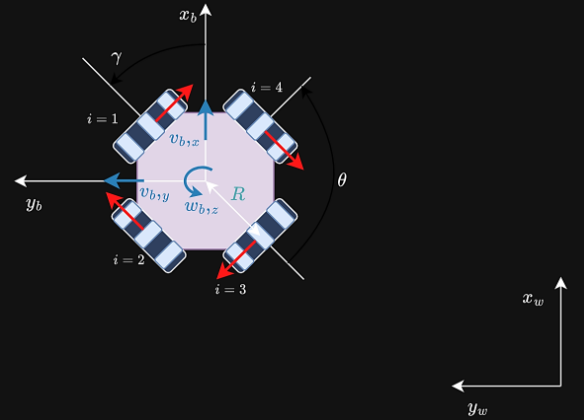
\includegraphics[width=0.65\linewidth]{figures/Chapter 5/Omni_kinematics.png}
    \caption{Omnidirectional Robot Coordinate Frames}
    \label{fig:omni_frames}
\end{figure}

\paragraph{World Frame $\{I\}$}
Fixed inertial frame with $(X_I, Y_I)$ horizontal and $Z_I$ upward. Robot pose: $\mathbf{q} = [x, y, \theta]^T$.

\paragraph{Robot Base Frame $\{B\}$}
Body-fixed frame at geometric center. $x_B$ forward, $y_B$ left, $z_B$ upward. Velocity:
\begin{equation}
\mathbf{v}_B = [v_{b,x}, v_{b,y}, \omega_{b,z}]^T
\label{eq:body_vel}
\end{equation}

\paragraph{Wheel Frames $\{W_i\}$}
Each wheel has driving angle $\alpha_i$ (orientation relative to $x_B$), position angle $\delta_i$ (angle from center to wheel), roller angle $\gamma$, and distance $R$ from robot center.

\subsubsection{Wheel Configuration}

The robot features three omni-wheels separated by 120°:

\begin{table}[H]
\centering
\caption{Three-Wheeled Omni Robot Configuration}
\label{tab:wheel_config}
\begin{tabular}{|l|c|c|c|}
\hline
\textbf{Parameter} & \textbf{Wheel 1} & \textbf{Wheel 2} & \textbf{Wheel 3} \\
\hline
Driving Angle $\alpha_i$ & 270° (--90°) & 150° & 30° \\
\hline
Position Angle $\delta_i$ & 0° & 240° (--120°) & 120° \\
\hline
Roller Angle $\gamma$ & \multicolumn{3}{c|}{0°} \\
\hline
Wheel Radius $r_w$ & \multicolumn{3}{c|}{0.034 m} \\
\hline
Base Radius $R$ & \multicolumn{3}{c|}{0.124 m} \\
\hline
\end{tabular}
\end{table}

\subsubsection{Inverse Kinematics}

The inverse kinematics transforms body velocities to wheel speeds. For a holonomic wheel, motor speed depends on:
\begin{itemize}
    \item \textbf{Longitudinal Velocity} ($v_t$): Motion along rolling direction
    \item \textbf{Lateral Velocity} ($v_p$): Sideways motion compensated by roller angle
\end{itemize}

The fundamental equation:
\begin{equation}
v_{wheel} = v_t + v_p \tan\gamma
\label{eq:wheel_fundamental}
\end{equation}

Velocity at wheel position:
\begin{equation}
\mathbf{v}_{q_{w_i}} = \begin{bmatrix} v_{b,x} + R\omega_{b,z}\sin\delta_i \\ v_{b,y} - R\omega_{b,z}\cos\delta_i \end{bmatrix}
\label{eq:wheel_pos_vel}
\end{equation}

Projecting onto wheel coordinates and simplifying for standard holonomic configuration ($\alpha_i - \delta_i = -90°$) with omni-wheels ($\gamma = 0°$):
\begin{equation}
\omega_i = \frac{1}{r_w} \begin{bmatrix} \cos\alpha_i & \sin\alpha_i & -R \end{bmatrix} \begin{bmatrix} v_{b,x} \\ v_{b,y} \\ \omega_{b,z} \end{bmatrix}
\label{eq:single_wheel_ik}
\end{equation}

The complete inverse kinematics matrix form:
\begin{equation}
\begin{bmatrix} \omega_1 \\ \omega_2 \\ \omega_3 \end{bmatrix} = \frac{1}{r_w} \begin{bmatrix} \cos\alpha_1 & \sin\alpha_1 & -R \\ \cos\alpha_2 & \sin\alpha_2 & -R \\ \cos\alpha_3 & \sin\alpha_3 & -R \end{bmatrix} \begin{bmatrix} v_{b,x} \\ v_{b,y} \\ \omega_{b,z} \end{bmatrix}
\label{eq:ik_general}
\end{equation}

Or in compact form: $\boldsymbol{\omega}_W = \frac{1}{r_w} \mathbf{H} \mathbf{v}_B = \mathbf{J}^{-1} \boldsymbol{\xi}$

Substituting configuration parameters:
\begin{equation}
\begin{bmatrix} \omega_1 \\ \omega_2 \\ \omega_3 \end{bmatrix} = \frac{1}{0.034} \begin{bmatrix} 0 & -1 & -0.124 \\ -\frac{\sqrt{3}}{2} & \frac{1}{2} & -0.124 \\ \frac{\sqrt{3}}{2} & \frac{1}{2} & -0.124 \end{bmatrix} \begin{bmatrix} v_{b,x} \\ v_{b,y} \\ \omega_{b,z} \end{bmatrix}
\label{eq:ik_numerical}
\end{equation}

\paragraph{Global Frame Transformation}
To use global velocities as input:
\begin{equation}
\begin{bmatrix} v_{b,x} \\ v_{b,y} \\ \omega_{b,z} \end{bmatrix} = \begin{bmatrix} \cos\theta & \sin\theta & 0 \\ -\sin\theta & \cos\theta & 0 \\ 0 & 0 & 1 \end{bmatrix} \begin{bmatrix} v_{i,x} \\ v_{i,y} \\ \omega_{i,z} \end{bmatrix}
\label{eq:frame_transform}
\end{equation}

\subsubsection{Forward Kinematics}

Forward kinematics estimates body velocity from measured wheel speeds by inverting the coefficient matrix:
\begin{equation}
\boldsymbol{\xi} = \mathbf{v}_B = r_w \mathbf{H}^{-1} \boldsymbol{\omega}_W = \mathbf{J} \boldsymbol{\omega}_W
\label{eq:fk_compact}
\end{equation}

The general form:
\begin{equation}
\begin{bmatrix} v_{b,x} \\ v_{b,y} \\ \omega_{b,z} \end{bmatrix} = r_w \begin{bmatrix} \frac{2}{3}\cos\alpha_1 & \frac{2}{3}\cos\alpha_2 & \frac{2}{3}\cos\alpha_3 \\ \frac{2}{3}\sin\alpha_1 & \frac{2}{3}\sin\alpha_2 & \frac{2}{3}\sin\alpha_3 \\ -\frac{1}{3R} & -\frac{1}{3R} & -\frac{1}{3R} \end{bmatrix} \begin{bmatrix} \omega_1 \\ \omega_2 \\ \omega_3 \end{bmatrix}
\label{eq:fk_general}
\end{equation}

Substituting configuration parameters:
\begin{equation}
\begin{bmatrix} v_{b,x} \\ v_{b,y} \\ \omega_{b,z} \end{bmatrix} = 0.034 \begin{bmatrix} 0 & -\frac{1}{\sqrt{3}} & \frac{1}{\sqrt{3}} \\ -\frac{2}{3} & \frac{1}{3} & \frac{1}{3} \\ -\frac{1}{0.372} & -\frac{1}{0.372} & -\frac{1}{0.372} \end{bmatrix} \begin{bmatrix} \omega_1 \\ \omega_2 \\ \omega_3 \end{bmatrix}
\label{eq:fk_numerical}
\end{equation}

\subsection{Omnidirectional Interface Driver}
\label{subsec:omni_interface_driver}

The omnidirectional interface driver provides the functional and probabilistic link between motion execution and state estimation. Beyond translating velocity commands into wheel actuation, it produces physically consistent odometry with meaningful uncertainty representation.

\subsubsection{Design Objectives}

The driver explicitly models motion uncertainty from encoder quantization, discretization effects, and execution errors. This enables:
\begin{itemize}
    \item Direct compatibility with probabilistic localization and sensor fusion frameworks
    \item Systematic alignment between simulated and real-world robot performance
    \item Consistent uncertainty propagation throughout the autonomy stack
\end{itemize}

\subsubsection{Functional Requirements}

\begin{enumerate}
    \item \textbf{Velocity Command Interface:} Receive planar velocities in robot body frame via standardized ROS 2 messages
    \item \textbf{Kinematic Transformation:} Map body velocities to wheel velocities supporting full holonomic motion
    \item \textbf{Wheel Command Generation:} Produce synchronized wheel commands for motor control
    \item \textbf{Uncertainty Modeling:} Account for wheel slip, actuator noise, and discretization effects
    \item \textbf{Covariance Propagation:} Compute motion covariance for odometry and sensor fusion
    \item \textbf{Odometry Feedback:} Publish pose increments with associated covariance
    \item \textbf{Real-Time Operation:} Process commands at rates sufficient for stable control
    \item \textbf{Safety Enforcement:} Enforce velocity and acceleration limits
\end{enumerate}

\subsubsection{Design Choices}

A custom driver was developed based on:
\begin{itemize}
    \item \textbf{White-Box Design:} All kinematic transformations, integration steps, and covariance propagation are explicitly implemented---critical for consistency between execution and estimation
    \item \textbf{Computational Efficiency:} Lightweight implementation preserves resources for SLAM and localization
    \item \textbf{Modularity:} Self-contained component with clearly defined interfaces
    \item \textbf{Extensibility:} External configuration of wheel geometry and noise characteristics
\end{itemize}

\subsubsection{Driver Architecture}

The ROS 2 node implements a layered structure:
\begin{enumerate}
    \item Command reception and validation
    \item Kinematic transformation (Eigen3 library)
    \item Odometry integration
    \item Covariance prediction
    \item Publication of wheel commands, odometry, and TF transforms
\end{enumerate}

\paragraph{Twist Representation}
Motion commands use planar twist:
\begin{equation}
\boldsymbol{\xi} = [v_x, v_y, \omega_z]^T
\label{eq:twist_rep}
\end{equation}
This abstraction decouples motion intent from mechanical implementation and provides a foundation for uncertainty propagation.

\paragraph{Kinematic Mapping}
The pipeline transforms twist to wheel velocities: $\boldsymbol{\omega}_w = \mathbf{J}^{-1} \boldsymbol{\xi}$

\subsubsection{Odometry Estimation}

\paragraph{Discrete-Time Integration}
Wheel encoder measurements are converted to incremental displacements and mapped to body-frame motion:
\begin{equation}
\Delta \mathbf{x}_b = [\Delta x, \Delta y, \Delta \theta]^T
\label{eq:body_increment}
\end{equation}

Using Euler integration, the global pose updates:
\begin{equation}
\mathbf{x}_{k+1} = \mathbf{x}_k + \mathbf{R}(\theta_k) \begin{bmatrix} \Delta x \\ \Delta y \end{bmatrix} + \begin{bmatrix} 0 \\ 0 \\ \Delta \theta \end{bmatrix}
\label{eq:euler_integration}
\end{equation}
where $\mathbf{R}(\theta_k)$ is the planar rotation matrix.

\paragraph{Coordinate Frames}
The driver publishes the \texttt{odom} $\rightarrow$ \texttt{base\_link} transform, representing estimated pose relative to a locally fixed reference. This continuous estimate is fused with global corrections from localization algorithms.

\subsubsection{Odometry Covariance Modeling}

\paragraph{Motivation}
Probabilistic localization (EKF, AMCL) requires accurate motion covariance. Deterministic odometry leads to overconfident predictions and estimator inconsistency.

\paragraph{Encoder Quantization Noise}
Each encoder provides discrete measurements with resolution defined by pulses per revolution (PPR). The smallest angular increment:
\begin{equation}
\Delta \phi = \frac{2\pi}{\text{PPR}}
\label{eq:encoder_resolution}
\end{equation}

Assuming uniform quantization, the angular measurement variance:
\begin{equation}
\sigma_\phi^2 = \frac{(\Delta \phi)^2}{12}
\label{eq:angular_variance}
\end{equation}

Propagated to wheel displacement:
\begin{equation}
\sigma_s^2 = r^2 \sigma_\phi^2
\label{eq:displacement_variance}
\end{equation}

\paragraph{Multi-Encoder Covariance}
For $N$ wheels with independent quantization noise:
\begin{equation}
\boldsymbol{\Sigma}_s = \text{diag}(\sigma_{s_1}^2, \sigma_{s_2}^2, \ldots, \sigma_{s_N}^2)
\label{eq:wheel_covariance}
\end{equation}

\paragraph{Robot Motion Uncertainty}
Through the forward kinematic Jacobian $\mathbf{J}$:
\begin{equation}
\boldsymbol{\Sigma}_{\Delta x} = \mathbf{J} \boldsymbol{\Sigma}_s \mathbf{J}^T
\label{eq:motion_covariance}
\end{equation}

This produces correlated uncertainty due to geometric coupling in omnidirectional platforms.

\paragraph{Twist Covariance}
For Kalman prediction, displacement covariance converts to velocity covariance:
\begin{equation}
\boldsymbol{\Sigma}_{\text{twist}} = \frac{1}{(\Delta t)^2} \boldsymbol{\Sigma}_{\Delta x}
\label{eq:twist_covariance}
\end{equation}

\subsubsection{Kalman Prediction for Covariance Propagation}

\paragraph{State Integration}
At each time step, the global pose updates:
\begin{align}
\Delta x &= (v_x \cos\theta_k - v_y \sin\theta_k) \Delta t \label{eq:delta_x} \\
\Delta y &= (v_x \sin\theta_k + v_y \cos\theta_k) \Delta t \label{eq:delta_y} \\
\Delta \theta &= \omega_z \Delta t \label{eq:delta_theta}
\end{align}

\paragraph{State Jacobian}
The Jacobian with respect to state $\mathbf{x} = [x, y, \theta]^T$:
\begin{equation}
\mathbf{F}_k = \begin{bmatrix} 1 & 0 & (-v_x \sin\theta_k - v_y \cos\theta_k) \Delta t \\ 0 & 1 & (v_x \cos\theta_k - v_y \sin\theta_k) \Delta t \\ 0 & 0 & 1 \end{bmatrix}
\label{eq:state_jacobian}
\end{equation}

\paragraph{Control Jacobian}
The Jacobian with respect to control $\mathbf{u}_k = [v_x, v_y, \omega_z]^T$:
\begin{equation}
\mathbf{G}_k = \begin{bmatrix} \cos\theta_k \Delta t & -\sin\theta_k \Delta t & 0 \\ \sin\theta_k \Delta t & \cos\theta_k \Delta t & 0 \\ 0 & 0 & \Delta t \end{bmatrix}
\label{eq:control_jacobian}
\end{equation}

\paragraph{Process Noise}
\begin{equation}
\mathbf{Q}_k = \mathbf{G}_k \boldsymbol{\Sigma}_{\text{twist}} \mathbf{G}_k^T
\label{eq:process_noise}
\end{equation}

\paragraph{Covariance Prediction}
\begin{equation}
\mathbf{P}_{k+1} = \mathbf{F}_k \mathbf{P}_k \mathbf{F}_k^T + \mathbf{Q}_k
\label{eq:covariance_prediction}
\end{equation}

This captures both propagation of existing uncertainty and injection of new uncertainty from motion execution. Higher $\mathbf{Q}_k$ indicates greater process model uncertainty.

The omnidirectional kinematic model enables heading-independent translation, a critical capability for navigation in cluttered environments. Simulation validation of this capability is presented in Section~\ref{subsec:omni_motion_validation}, demonstrating pure lateral motion while maintaining constant heading.
\newpage
\section{Autonomous System Node Structure}
\label{sec:autonomous_system_nodes}

This section provides a consolidated view of the complete autonomous system architecture, synthesizing the individual components described throughout this chapter into a unified data flow diagram.

\subsection{Single Robot Architecture}

A detailed breakdown of the internal software pipeline for a single robot instance is shown in Figure \ref{fig:deep_dive}. This diagram illustrates the three-layer architecture: Perception, Autonomy, and Control.

\begin{figure}[H]
    \centering
    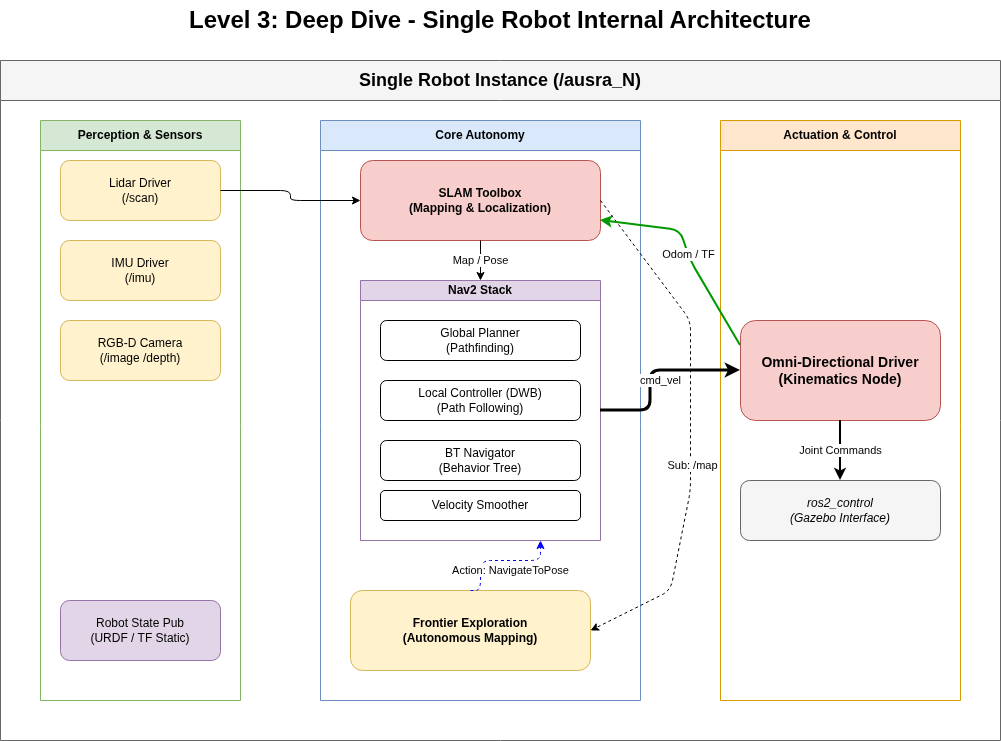
\includegraphics[width=0.95\linewidth]{figures/Chapter 5/Deep_dive_single_robot.png}
    \caption{Level 3: Deep Dive - Single Robot Internal Architecture}
    \label{fig:deep_dive}
\end{figure}

\subsection{Data Flow Pipeline}

\subsubsection{Perception Layer}
The perception layer acquires and processes raw sensor data:
\begin{itemize}
    \item \textbf{LiDAR Driver:} Publishes 2D laser scans at 5.5 Hz on \texttt{/scan}
    \item \textbf{IMU Driver:} Publishes inertial data at 100 Hz on \texttt{/imu/data\_raw}
    \item \textbf{Depth Camera:} Publishes point clouds and RGB images for obstacle detection
    \item \textbf{Wheel Encoders:} Provide tick counts to the omni\_driver for odometry computation
\end{itemize}

\subsubsection{Localization and Mapping Layer}
This layer fuses sensor data to build environmental understanding:
\begin{itemize}
    \item \textbf{EKF Node:} Fuses IMU and wheel odometry to produce filtered state estimates on \texttt{/odometry/filtered}
    \item \textbf{SLAM Toolbox:} Consumes laser scans and odometry to build the occupancy grid map and refine robot pose through scan matching
    \item \textbf{TF Broadcaster:} Maintains the transform tree connecting all coordinate frames
\end{itemize}

\subsubsection{Planning and Navigation Layer}
The Nav2 stack handles high-level decision making:
\begin{itemize}
    \item \textbf{Behavior Tree Navigator:} Orchestrates the navigation task using a behavior tree, handling recovery actions and goal management
    \item \textbf{Planner Server (SmacPlanner2D):} Computes globally optimal paths using A* search on the costmap
    \item \textbf{Controller Server (DWB):} Generates local trajectories that follow the global path while avoiding dynamic obstacles
    \item \textbf{Costmap 2D:} Maintains layered costmaps (static, obstacle, inflation) for planning
\end{itemize}

\subsubsection{Control Layer}
The control layer executes velocity commands:
\begin{itemize}
    \item \textbf{Omni Driver:} Converts body-frame velocities ($v_x$, $v_y$, $\omega$) to wheel angular velocities using the inverse kinematics matrix (Equation \ref{eq:ik_general})
    \item \textbf{micro-ROS Agent:} Bridges ROS 2 DDS to the ESP32 via UART at 921600 baud
    \item \textbf{ESP32 Firmware:} Executes PID control loops for each motor at 100 Hz
\end{itemize}

\subsection{Topic Summary}

Table \ref{tab:topic_summary} provides a comprehensive list of the key ROS 2 topics in the autonomous system.

\begin{table}[H]
\centering
\caption{Autonomous System Topic Summary}
\label{tab:topic_summary}
\begin{tabular}{|l|l|c|l|}
\hline
\textbf{Topic} & \textbf{Message Type} & \textbf{Rate} & \textbf{Purpose} \\
\hline
\texttt{/scan} & sensor\_msgs/LaserScan & 5.5 Hz & LiDAR data \\
\texttt{/imu/data\_raw} & sensor\_msgs/Imu & 100 Hz & IMU measurements \\
\texttt{/odometry/filtered} & nav\_msgs/Odometry & 50 Hz & EKF state estimate \\
\texttt{/map} & nav\_msgs/OccupancyGrid & 1 Hz & SLAM output \\
\texttt{/goal\_pose} & geometry\_msgs/PoseStamped & Event & Navigation goal \\
\texttt{/plan} & nav\_msgs/Path & Event & Global path \\
\texttt{/cmd\_vel} & geometry\_msgs/Twist & 20 Hz & Velocity command \\
\texttt{/wheel/odom} & nav\_msgs/Odometry & 100 Hz & Wheel odometry \\
\texttt{/tf} & tf2\_msgs/TFMessage & 100 Hz & Transform tree \\
\hline
\end{tabular}
\end{table}

The complete autonomous stack integrating all these components was validated through comprehensive simulation testing, achieving 95\% map coverage in under 1 minute 40 seconds. Detailed integration test results are presented in Section~\ref{subsec:complete_stack_test}.

\section{Robot Description (URDF)}
\label{sec:urdf}

The physical description of the robot is defined using the Unified Robot Description Format (URDF), augmented by the Xacro macro system for modularity and multi-robot support.

\subsection{Xacro Architecture}

The robot description is split into modular files:
\begin{itemize}
    \item \texttt{robot.urdf.xacro}: Top-level entry point accepting arguments (e.g., \texttt{robot\_name}) and including sub-components
    \item \texttt{robot\_core.xacro}: Defines physical chassis, wheels, and joints with dynamic namespacing support
    \item \texttt{sensors.xacro}: Attaches sensor plugins (LiDAR, Camera, IMU) to the base link
    \item \texttt{gazebo\_classic.xacro}: Defines Gazebo-specific tags (friction, materials) and loads \texttt{ros\_control} plugins
\end{itemize}

\subsection{Model Generation}

At runtime, the Xacro engine generates pure XML URDF. For example, spawning \texttt{ausra\_1}:
\begin{verbatim}
xacro robot.urdf.xacro robot_name:=ausra_1
\end{verbatim}

This replaces all \texttt{\$\{robot\_name\}} occurrences with \texttt{ausra\_1}, creating a unique TF tree (e.g., \texttt{ausra\_1\_base\_link}, \texttt{ausra\_1\_wheel\_1}) that allows multiple robots to coexist in the same TF buffer.

See Appendix \ref{app:urdf_code} for the core chassis definition.

\section{Future Work and Research}
\label{sec:ch5_future_work}

The architecture is designed to support advanced collaborative features currently in research and development.

\subsection{Collaborative Algorithms (Planned)}

\begin{itemize}
    \item \textbf{Single Pose Graph SLAM:} All robots contribute to a unified constraint graph, allowing Loop Closures triggered by Agent A to correct Agent B's pose drift, creating a mathematically consistent global map
    \item \textbf{mTSP Task Allocation:} Integration of a centralized ``Multiple Traveling Salesman Problem'' solver (using Google OR-Tools) to replace frontier assignment with globally optimal scheduling, minimizing total coverage time
    \item \textbf{Lazy Traffic Controller:} Decentralized avoidance using ``Velocity Obstacles'' where agents broadcast velocity vectors to neighbors, computing collision-free trajectories in velocity space without central planning
\end{itemize}

\subsection{Advanced Perception}

Future upgrades include:
\begin{itemize}
    \item Inter-Process Communication (IPC) for high-frequency camera data handling
    \item AprilTag detection for automated victim identification and localization
\end{itemize}

